\documentclass[UTF8,a4paper]{ctexart}
\usepackage[margin=1in]{geometry}
\usepackage{fancyhdr,hyperref,float,graphicx,amsmath}
\pagestyle{fancy}
\hypersetup{hidelinks}

\lhead{\bfseries \leftmark}
\chead{}
\rhead{SCUT}
\lfoot{\url{https://github.com/285571052}}
\cfoot{qhy}
\rfoot{\thepage}
\setlength{\headheight}{13pt}
\renewcommand{\headrulewidth}{0.4pt}
\renewcommand{\footrulewidth}{0.4pt}

\setlength{\parindent}{0pt}
\newcommand{\spaceline}{\vspace{\baselineskip}}

\author{ qhy }
\date{\today}
\title{高性能计算与云计算}

\begin{document}
  \maketitle
  \tableofcontents
  \newpage

  \section{介绍}

  \textbf{高性能与云计算关注的问题:}\\
  如何使计算机更快更方便地解决更大规模的问题。

  \spaceline
  \textbf{做得更快的方法:}
  \begin{enumerate}
    \item [1.] work harder:换一台更好的计算机

    \item [2.] work smarter:修改为更加优化的方法

    \item [3.] getting help:并行处理
  \end{enumerate}

  单核CPU的提升遇到瓶颈,提高计算机性能需要另寻出路:多核时代,由AMD首先推出。

  \spaceline
  \textbf{多核运算的速度一定比单核的CPU快吗?}\\
  不一定,考虑到散热等问题,多核CPU的主频往往比单核的低,若程序只能发挥出一个内核效用的话,
  自然不如单核CPU快。\\
  想要发挥多核功能,设计的软件首先要做并行运算。\\
  多核的出现,使得高性能计算进入普及时代。

  \spaceline
  \textbf{大规模数据处理当前面临的问题:}
  \begin{enumerate}
    \item [1.] 大规模PC集群可靠性差

    一台PC的MTBF(Mean Time Between Failure) = 3年

    则1000台PC的MTBF = 1天

    商用网络 = 低带宽

    这个要求运行系统具备良好的可扩展性、良好的容错能力

    \item [2.] 并行/分布式程序开发、调试困难

    \begin{enumerate}
      \item 数据划分
      \item 任务调度
      \item 任务之间的通信
      \item 错误的处理、容错
    \end{enumerate}

    这要求编程模型具备一定表达能力、很好的简单易用性
  \end{enumerate}

  大数据时代的高性能计算:云计算:通过互联网将资源按需服务的形式提供给用户。

  \spaceline
  \textbf{课程内容}
  \begin{enumerate}
    \item 高性能计算系统与其结构模型
    \item 并行算法设计
    \item 并行程序的设计原理和方法
    \item 云计算
    \item 高性能计算与云计算的应用及发展趋势
  \end{enumerate}

  \spaceline
  \textbf{高性能计算与云计算的3大基础:}
  \begin{enumerate}
    \item 计算:数据处理能力

    \item 存储

    \item 通信
  \end{enumerate}

  \spaceline
  \textbf{高性能计算与分布式计算的区别?}\\
  高性能计算是把计算任务分配到各个节点上计算\\
  分布式计算则是把各种资源分布在各个节点上计算

  \textbf{高性能计算的应用领域}:密码解密, 大规模数据分析 ,天气预报 ,搜索引擎 ,工程高性能计算 , 动漫与影视创作 , 商业智能 , 计算药学 , 计算科学

  \textbf{高性能计算应用分类}:计算密集型 , 数据密集型 , 网络密集型

  \textbf{云计算}:通过互联网将资源以"按需服务"的形式提供给用户

  \textbf{云计算的特点:}分布式 , 虚拟化 , 动态可扩展

  \begin{figure}[H]
    \centering
    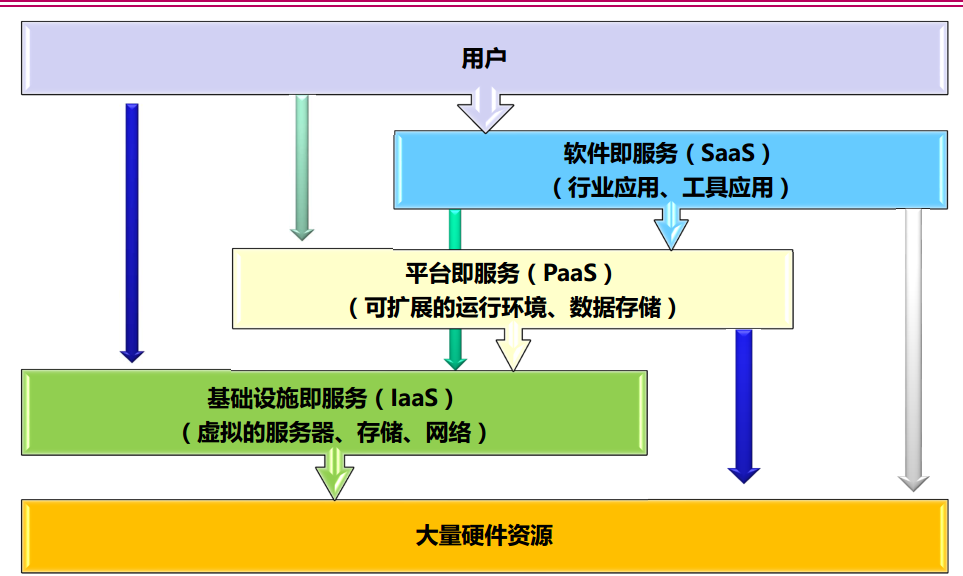
\includegraphics[scale = 0.3]{assets/ParallelComputing_e82fe.png}
    \caption{云计算服务的层次}
  \end{figure}

  \textbf{高性能计算与云计算的共同点:}都是大规模系统, 相同的核心技术和挑战

  \textbf{高性能计算与云计算的区别:}
  \begin{itemize}
    \item 应用:高性能计算面向科学计算 、工程模拟 ,动漫渲染等领域 , 大多属于 计算密集型应用
    \\云计算主要是在 社交网络 、企业IT建设和信息化等领域 , 以 数据密集新 、 I/O密集型应用为主
    \item 技术:HPC需要特制的高速互连网络,而几乎不用虚拟化技术 ,而在云计算中,虚拟化技术是最基础的技术
    \item 用户:高性能计算主要面向政府部门,大企业 专业人士 , 而云计算具有良好的用户界面, 面向各种企业及普通用户
  \end{itemize}

  % \spaceline
  % \textbf{高性能计算的模型框架???没记录,名字也不确定对不对}
  \section{并行计算机体系结构}
  大部分并行计算机都是MIMD系统:
  \begin{itemize}
    \item PVP Paraller Vector Processor
    \item SMP Symmetric Multiprocessors
    \item MPP Massively Parallel Multiprocessors
    \item DSM Distributed Shared Memory
    \item 集群 Cluster
    \item 分布式系统 Distributed Systems
  \end{itemize}

  可分为两种架构:\textbf{多处理器架构 Multiprocessors} ; \textbf{多计算机架构 Multicomputers}

  \begin{itemize}
    \item 多处理器:共享存储空间
    \begin{itemize}
      \item PVP : 高性能矢量处理器通过高带宽的交叉开关连接在一起
      \item SMP : 商业微处理器通过高速总线或交叉开关\\
      对称性:共享存储 , 单地址空间\\
      问题:可靠性差 , 通信延迟(相比CPU) , 带宽增加缓慢 , 不可扩放($\to$CC-NUMA)
      \item DSM : 与SMP 类似,但存储是物理分布在每个节点
    \end{itemize}
    \begin{figure}[H]
      \centering
      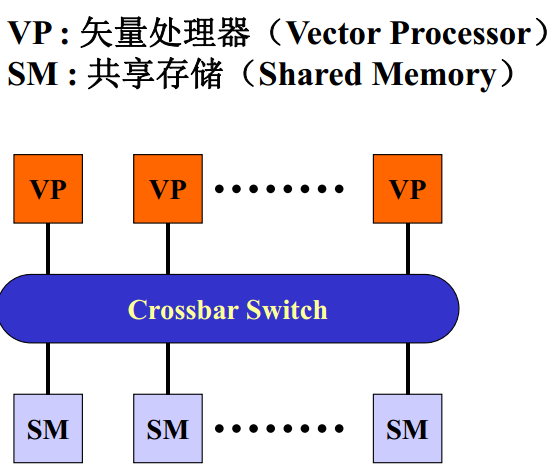
\includegraphics[scale = 0.3]{assets/ParallelComputing_11aed.png}
      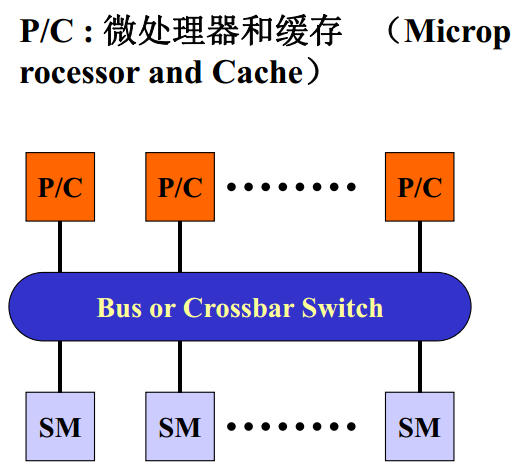
\includegraphics[scale = 0.3]{assets/ParallelComputing_2b522.png}
      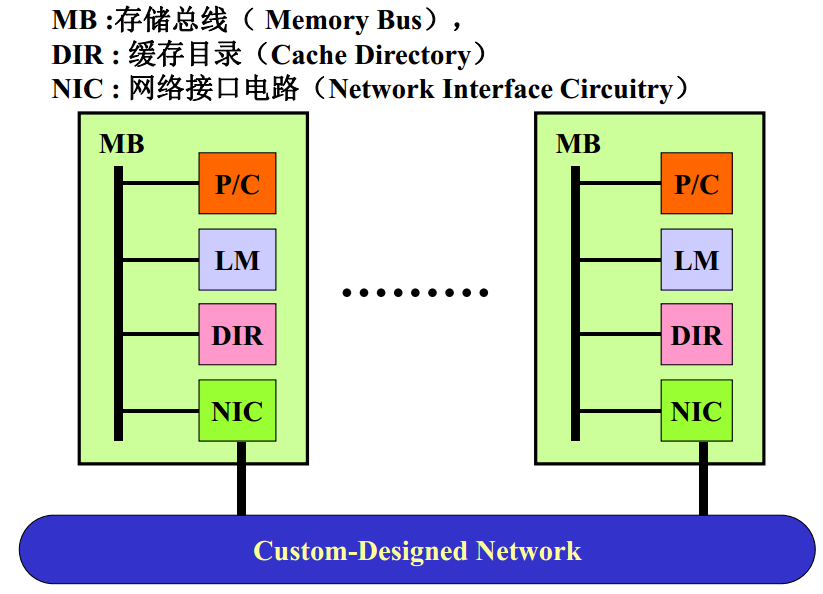
\includegraphics[scale = 0.3]{assets/ParallelComputing_181a4.png}
      \caption{PVP , SMP . DSM}
    \end{figure}
    \item 多计算机架构 : 消息传递结构
    \begin{itemize}
      \item MPP : 处理器总数目$>$ 1000
      \item Cluster : 系统中的每个节点的处理器少于16个
      \item Constellation : 系统中的每个节点的处理器多于16个
    \end{itemize}
    \begin{figure}[H]
      \centering
      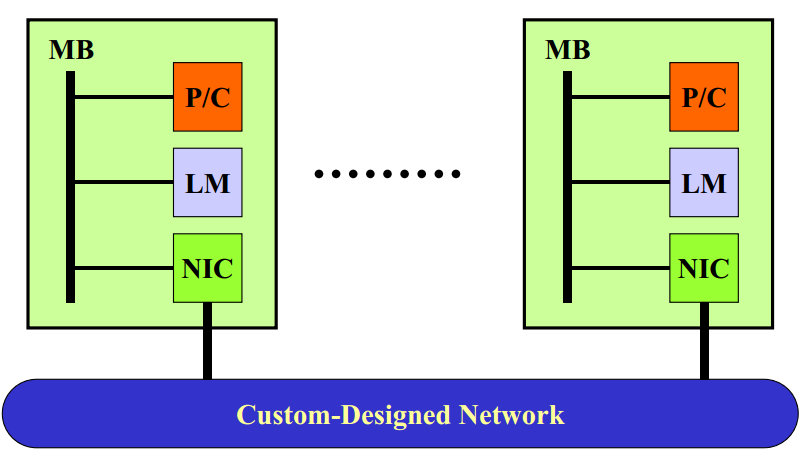
\includegraphics[scale = 0.2]{assets/ParallelComputing_5234c.png}
      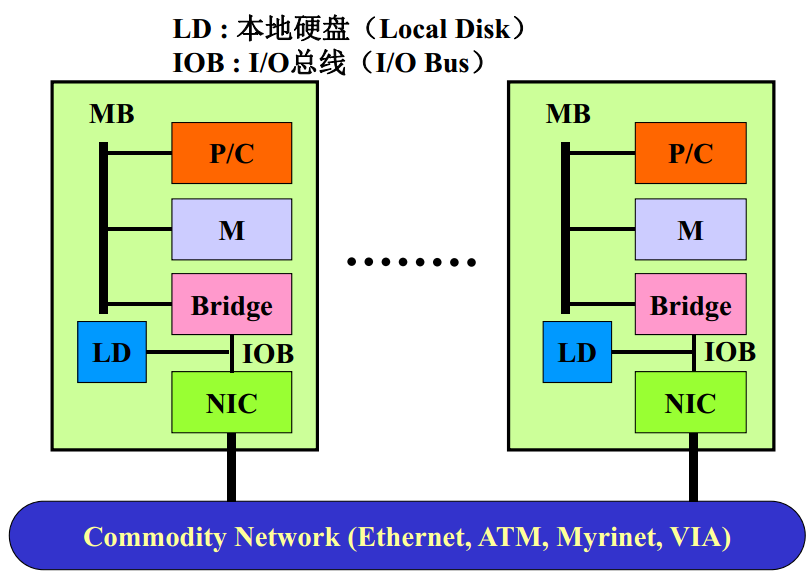
\includegraphics[scale = 0.2]{assets/ParallelComputing_3eb47.png}
      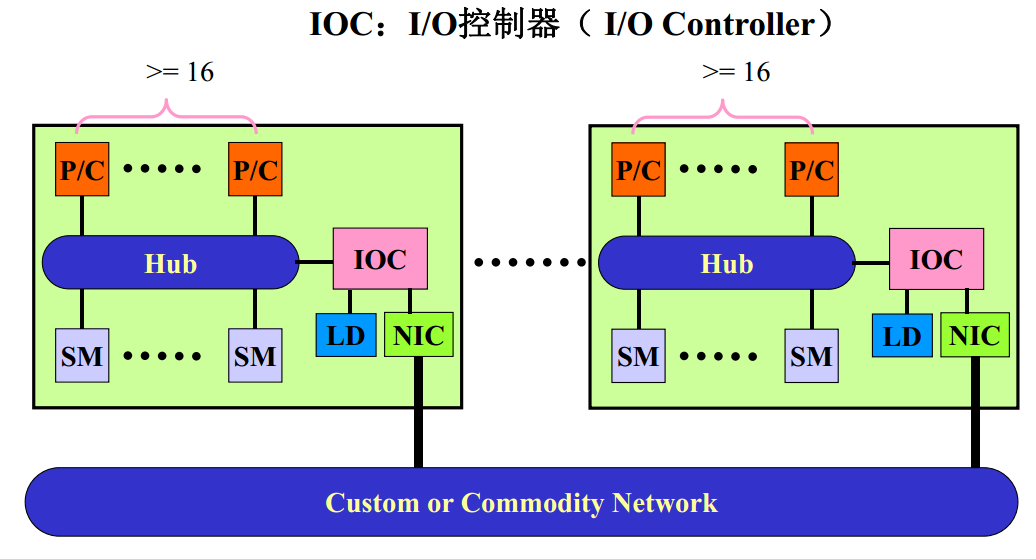
\includegraphics[scale = 0.3]{assets/ParallelComputing_04d17.png}
      \caption{MPP , Cluster , Constellation}
    \end{figure}
  \end{itemize}

  \subsection{并行计算机系统}
  3类:SMP MPP 集群

  \textbf{工作站集群 COW}: 每分布式存储 , 每个节点都是完整的计算机(MPP只有微内核)

  \textbf{集群与分布式系统的区别}:
  \begin{itemize}
    \item 集群继承了分布式系统的大部分只是
    \item 分布式系统通常是一个计算机的动物园,具有许多不同种类的计算机
    \item 集群通常是同构的,耦合度较紧密, 节点间互为信任关系
  \end{itemize}
  \begin{figure}[H]
    \centering
    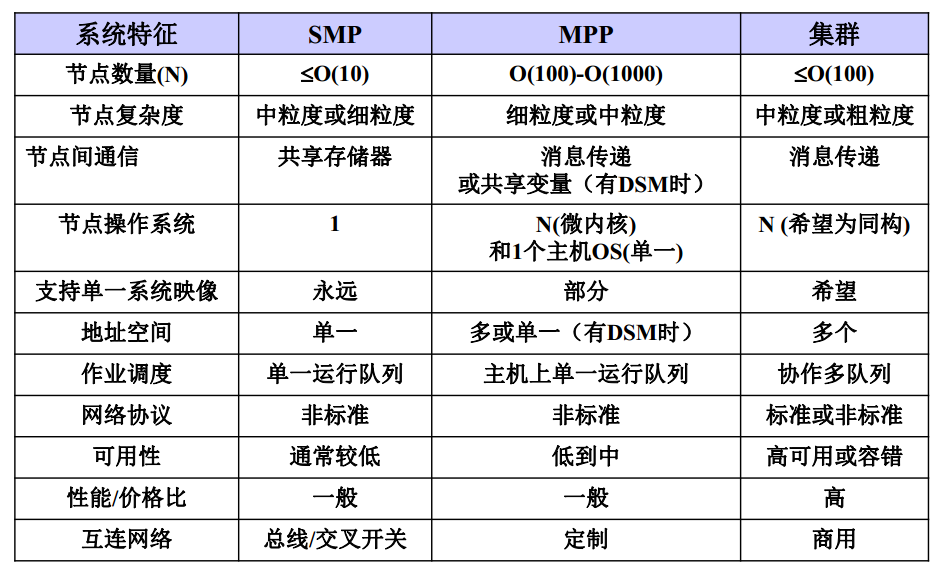
\includegraphics[scale = 0.3]{assets/ParallelComputing_4c4bb.png}
    \caption{SMP 、 MPP 、 集群 的比较}
  \end{figure}

  \section{并行结构}
  并行计算机与传统计算机的区别在于其通信架构。\\
  并行计算机的发展体现在:
  \begin{itemize}
    \item 计算节点性能的提高
    \item 节点之间通信的改进
  \end{itemize}

  \begin{figure}[H]
    \centering
    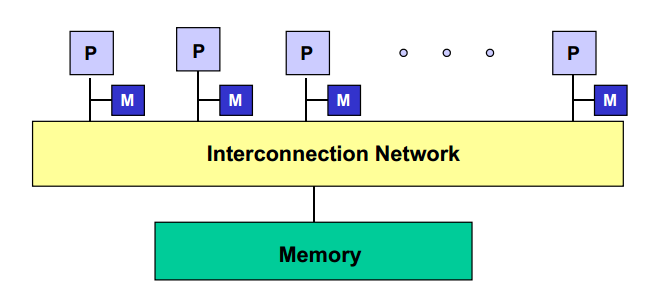
\includegraphics[scale = 0.3]{assets/ParallelComputing_0293e.png}
    \caption{一个通用的并行结构:P表示处理器, M表示本地内存,Memory表示共享内存}
  \end{figure}

  \spaceline
  \textbf{时延:}软件开销 + 通信时延+ 选路时延+ 竞争时延\\
  竞争时延:网络阻塞的时候需要等待。\\
  传输时延:通信时延 + 选路时延

  \spaceline
  \textbf{带宽:}
  \begin{itemize}
    \item 端口带宽\\
    从任意端口到另外端口单位时间内传送消息的最大位数
    \item 聚集带宽\\
    从一半节点到另一半节点,单位时间内传输消息的最大位数
    \item 链路带宽\\
    单位时间内链路传输消息的最大位数
    \item 对剖带宽\\
    每秒钟内,在最小的对剖平面上通过所有连线的最大信息位数。\\
    对剖带宽 = 对剖宽度\footnote{对剖宽度:将网络分成两个相等部分所必须移去的最少边数。
    对剖宽度越大越好,这样当某个节点故障的时候,整个网络瘫痪的几率就越小} $\times$ 链路带宽
  \end{itemize}

  \spaceline
  \textbf{互联网络的评价标准:}
  \begin{itemize}
    \item 硬件复杂度(Cost):将N个处理机按一定拓扑结构连成网络所需要的开关的个数
    \item 时延(Latency):发送消息到接受消息所需的时间
    \item 可扩展性
    \item 容错能力
    \item 带宽:单位时间内传送的数据量
  \end{itemize}


  \subsection{静态互连网络与动态互连网络}
  \textbf{静态互连网络:}处理单元之间的连接是固定的。
  \begin{itemize}
    \item 一维线性阵列
    \begin{figure}[H]
      \centering
      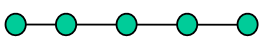
\includegraphics[scale = 0.3]{assets/ParallelComputing_c8f8c.png}
      \caption{一维线性阵列:线,直径:$N-1$,对剖宽度:$1$}
    \end{figure}
    \begin{figure}[H]
      \centering
      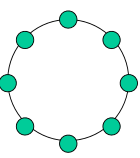
\includegraphics[scale = 0.3]{assets/ParallelComputing_b1923.png}
      \caption{一维线性阵列:环,直径:$\lfloor\frac{N}{2}\rfloor$,对剖宽度:$ 2 $}
    \end{figure}
    \item 二维网孔
    \begin{figure}[H]
      \centering
      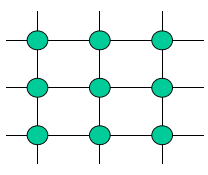
\includegraphics[scale = 0.3]{assets/ParallelComputing_ea5ca.png}
      \caption{二维网孔:网络规模:$N$ , 直径:$2(N^{\frac{1}{2}} - 1)$ , 对剖宽度:$N^{\frac{1}{2}}$}
    \end{figure}
    \begin{figure}[H]
      \centering
      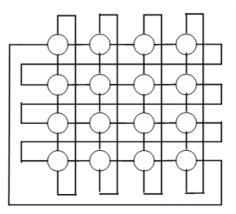
\includegraphics[scale = 0.3]{assets/ParallelComputing_5b5f4.png}
      \caption{Illiac 网孔:垂直方向上带环绕,水平方向呈蛇形状,
      网络规模:$N$ , 直径:$N^{\frac{1}{2}} - 1$ , 对剖宽度:$2N^{\frac{1}{2}}$}
    \end{figure}
    \begin{figure}[H]
      \centering
      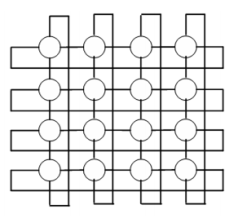
\includegraphics[scale = 0.3]{assets/ParallelComputing_d6701.png}
      \caption{2D环绕:垂直方向和水平方向都带环绕。
      网络规模:$N$ , 直径:$2\lfloor \frac{N^{\frac{1}{2}}}{2} \rfloor$ , 对剖宽度:$2N^{\frac{1}{2}}$}
    \end{figure}
    \item 树\\
    \textbf{星型网络:}是树的一个特殊情况。\\
    \textbf{胖树:}传统多叉树,根节点容易成为通信的瓶颈,因为带宽不够,胖树则是越靠近根带宽越大。
    \begin{figure}[H]
      \centering
      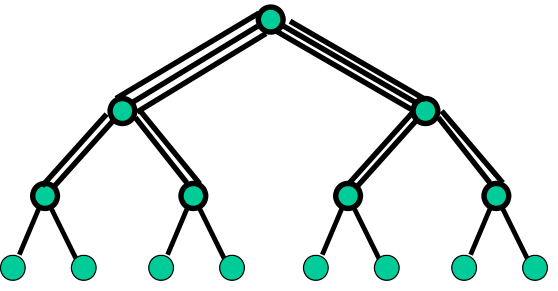
\includegraphics[scale = 0.3]{assets/ParallelComputing_3e1c8.png}
      \caption{Fat-Trees}
    \end{figure}
    \item 超立方\\
    一个n-立方由$N = 2^n$个顶点组成。直径为$n$,对剖宽度为$\frac{N}{2}$
    \begin{figure}[H]
      \centering
      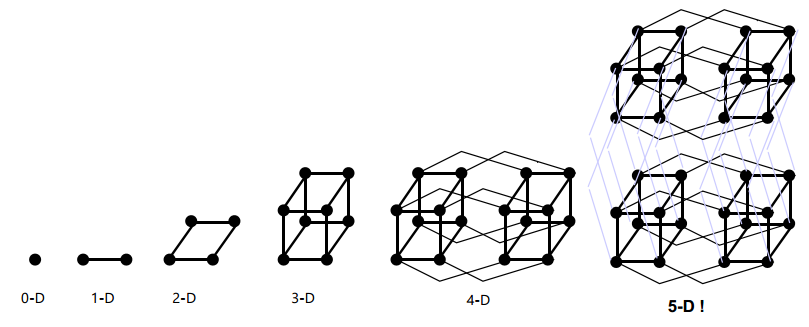
\includegraphics[scale = 0.3]{assets/ParallelComputing_9924c.png}
      \caption{超立方}
    \end{figure}
    \item 立方环\\
    将超立方上的节点使用一个环代替。
    \begin{figure}[H]
      \centering
      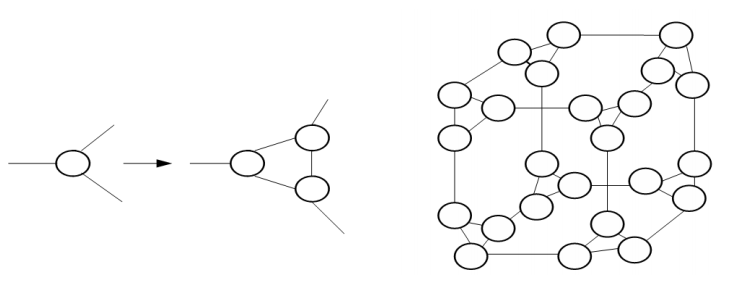
\includegraphics[scale = 0.3]{assets/ParallelComputing_b9cb4.png}
      \caption{3-立方环}
    \end{figure}
    \item 蝶形网络
    \begin{figure}[H]
      \centering
      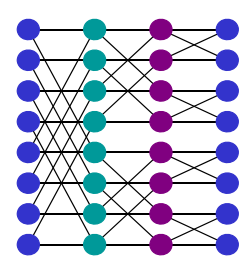
\includegraphics[scale = 0.4]{assets/ParallelComputing_00400.png}
      \caption{蝶网:规模:$N = (k+1)2^k$ , 直径:$2k$ , 对剖宽度:$2^k$}
    \end{figure}

  \end{itemize}

  \begin{figure}[H]
    \centering
    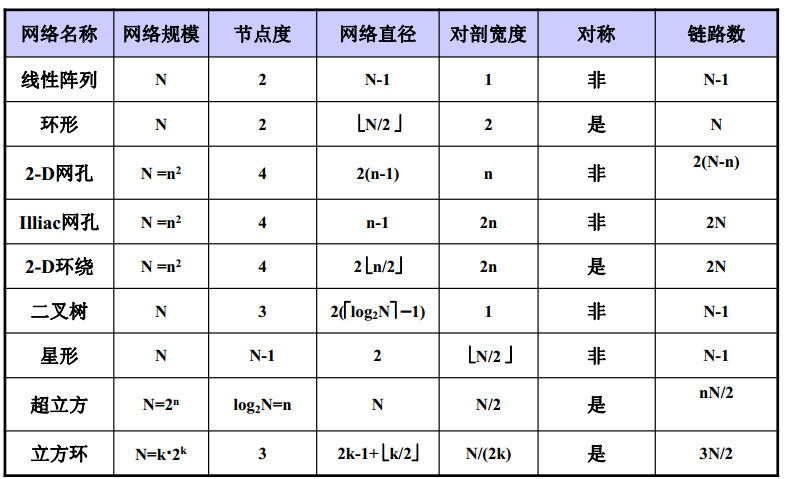
\includegraphics[scale = 0.5]{assets/ParallelComputing_3087c.png}
    \caption{静态互联网络特性比较}
  \end{figure}

  \textbf{小结:}
  \begin{itemize}
    \item 节点度越大,连接性越好,但网络越复杂,成本越高
    \item 一般静态网络节点度小于4
    \item 对剖宽度越大越好
    \item 网络尽可能对称,这样便于管理
    \item 对称性影响可扩展性与路由效率
  \end{itemize}

  \spaceline
  \textbf{动态互连网络:}连接可以动态地变换,用交换开关构建。
  \begin{itemize}
    \item 总线\\
    成本低,不随处理器数目的增加而增加\\
    扩展性不好,总线的带宽固定,随着处理器数增多,每个处理器带宽减少\\
    可利用程序中的局部性原理减少对总线带宽的需求
    \item 多叉开关\\
    任意两点之间有一个开关,对应两个状态on和off\\
    具备良好的宽带特性,带宽独享,完全非阻塞通讯\\
    但是代价大$O(n^2)$\\
    有两种使用方式,一:处理器间通信,二:处理器和存储模块之间的存取
    \item 多级互连网络\\
    多个交叉开关级联起来\\
    \textbf{交换开关模块}:允许一对多的连接,但不允许多对一的连接(即单一方向)
  \end{itemize}

  \begin{figure}[H]
    \centering
    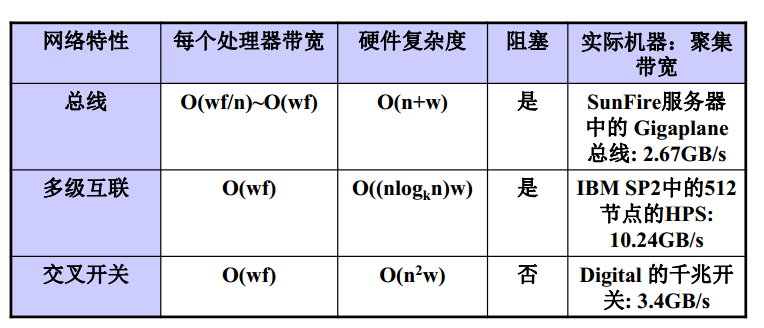
\includegraphics[scale = 0.5]{assets/ParallelComputing_3cbfc.png}
    \caption{动态互联网络比较,n:节点规模,w:数据宽度,f:时钟频率}
  \end{figure}

  \spaceline
  \textbf{标准互联网络}
  \begin{itemize}
    \item 以太网
    \item InfiniBand
  \end{itemize}

  \section{存储模型}
  \subsection{访存模型}
  访存模型类型:\textbf{共享存储 (多处理器架构)} , \textbf{分布式存储 (多计算机架构)}

  \begin{figure}[H]
    \centering
    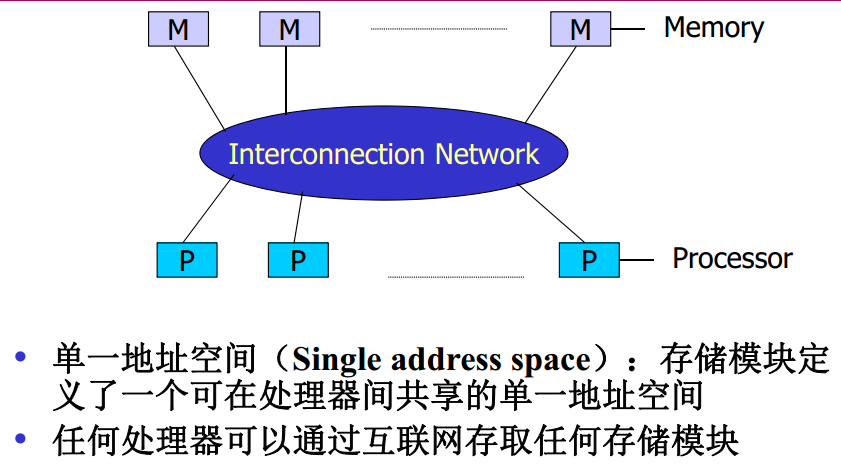
\includegraphics[scale = 0.3]{assets/ParallelComputing_b2071.png}
    \caption{共享存储}
  \end{figure}

  \begin{figure}[H]
    \centering
    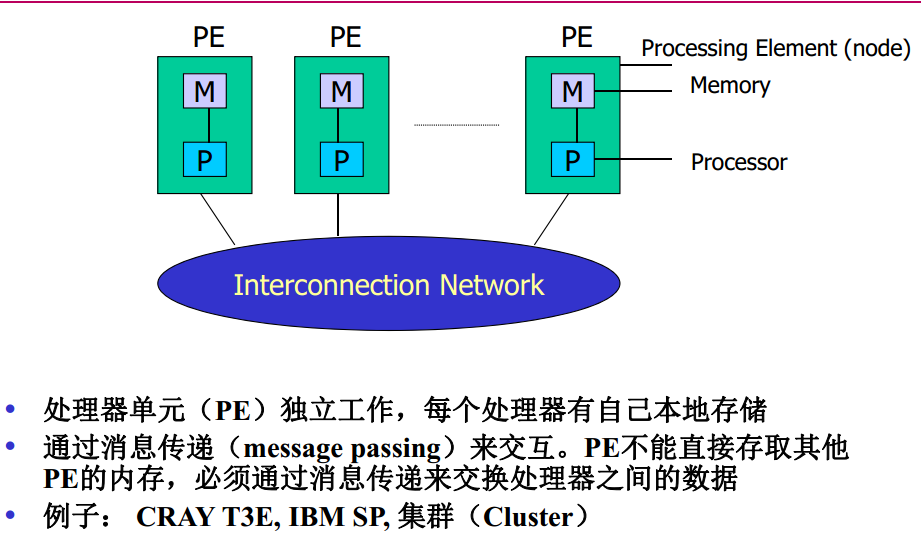
\includegraphics[scale = 0.3]{assets/ParallelComputing_ed9df.png}
    \caption{分布式存储}
  \end{figure}

  \textbf{存储器结构分类}: \textbf{集中式存储器} 、 \textbf{分布式存储器}
  \begin{itemize}
    \item 集中式存储器 : UMA Uniform Memory Access
    \begin{figure}[H]
      \centering
      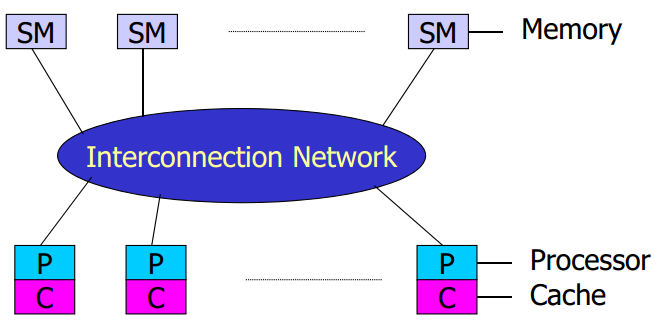
\includegraphics[scale = 0.3]{assets/ParallelComputing_c3b59.png}
      \caption{UMA}
    \end{figure}
    UMA,均匀存储模型 : 物理存储器被所有处理器均匀共享 , 访存时间相同 , 每个处理器带有高速缓存 , 外围设备也可以一定形式共享
    \item 分布式存储器
    \begin{itemize}
      \item NUMA Non-Uniform Memory Access\\
      NCC-NUMA,Non Cache Coherent NUMA; COMA , Cache Only Memory Architecture ; CC-NUMA Cache Coherent NUMA
    \end{itemize}
    \begin{figure}[H]
      \centering
      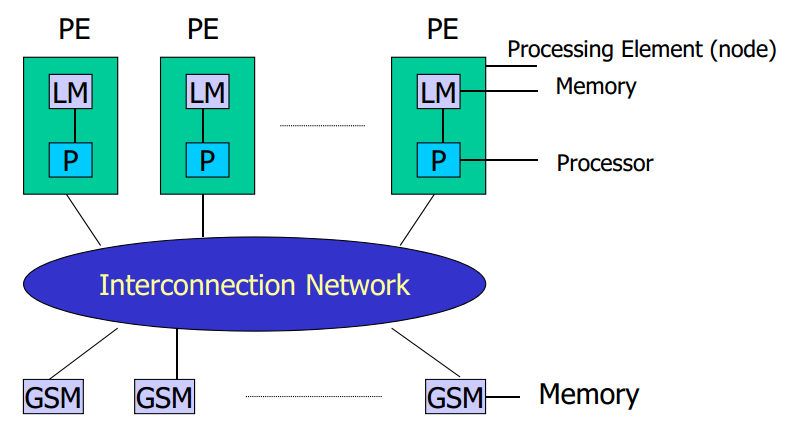
\includegraphics[scale = 0.3]{assets/ParallelComputing_1d9bd.png}
      \caption{NCC-NUMA}
    \end{figure}
      NCC-NUMA 非均匀存储访问模型 : 共享的存储器物理分布在每个处理器中, 本地存储器的集合构成全局地址空间 , 因此, 处理器访存时间是不一致的 , 每台处理器可以带有告诉缓存 ,外设也可以某种形式共享\\
      存储物理上是分布的,在逻辑上是全局可取的

      \begin{figure}[H]
        \centering
        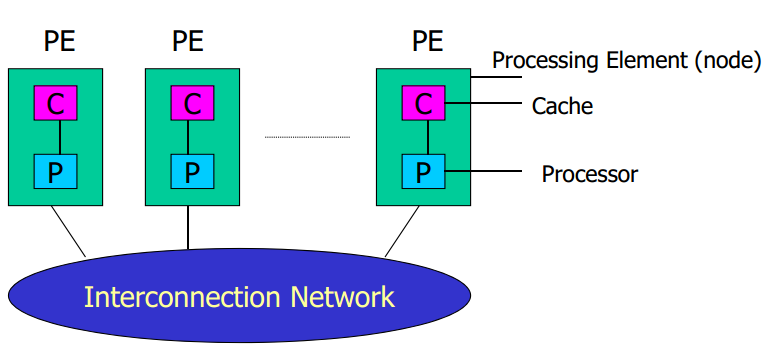
\includegraphics[scale = 0.3]{assets/ParallelComputing_eb08a.png}
        \caption{COMA}
      \end{figure}
      COMA 高速缓存存储访问模型 : 没有存储层次结构 ,全部高速缓存组成全局地址空间 , 利用分布的告诉缓存目录进行远程告诉缓存访问 , COMA没有物理地址

      \begin{figure}[H]
        \centering
        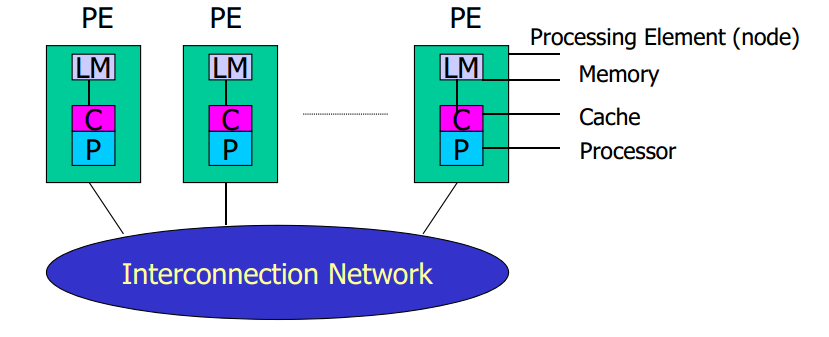
\includegraphics[scale = 0.3]{assets/ParallelComputing_88c48.png}
        \caption{CC-NUMA}
      \end{figure}
      CC-NUMA 高速缓存一致性非均匀鵆模型 : NUMA + Cache , 大多数使用基于目录的高速缓存一致性协议 , 保留SMP结构易于编程的有点, 也改善SMP的可扩放性


    \item NORMA : 非远程存储访问模型 , 所有存储器都是私有的,节点不能访问远程存储器 ,必须通过 \textbf{消息传递} 方式
    \begin{figure}[H]
      \centering
      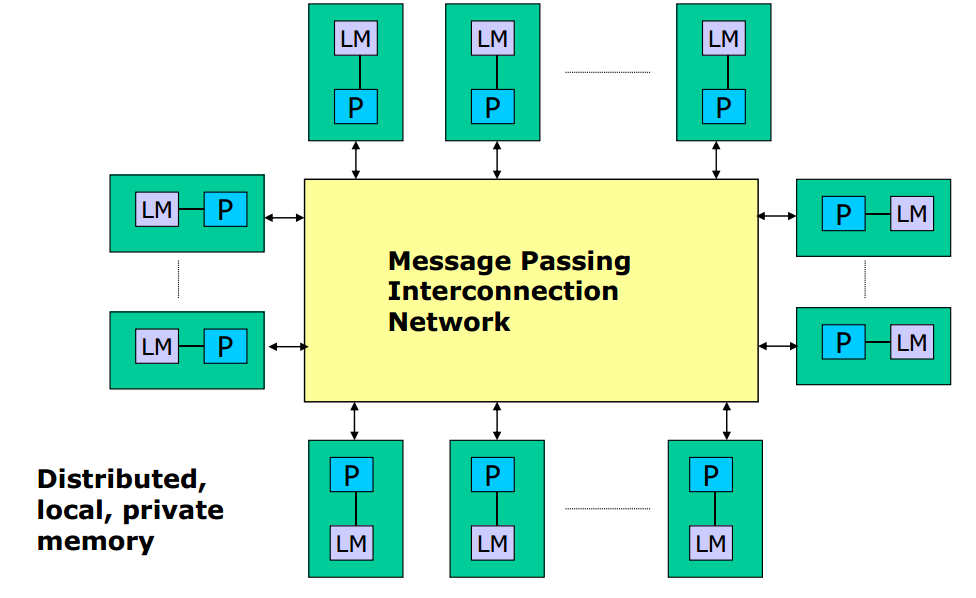
\includegraphics[scale = 0.3]{assets/ParallelComputing_cb17b.png}
      \caption{NORMA}
    \end{figure}
  \end{itemize}
  \begin{figure}[H]
    \centering
    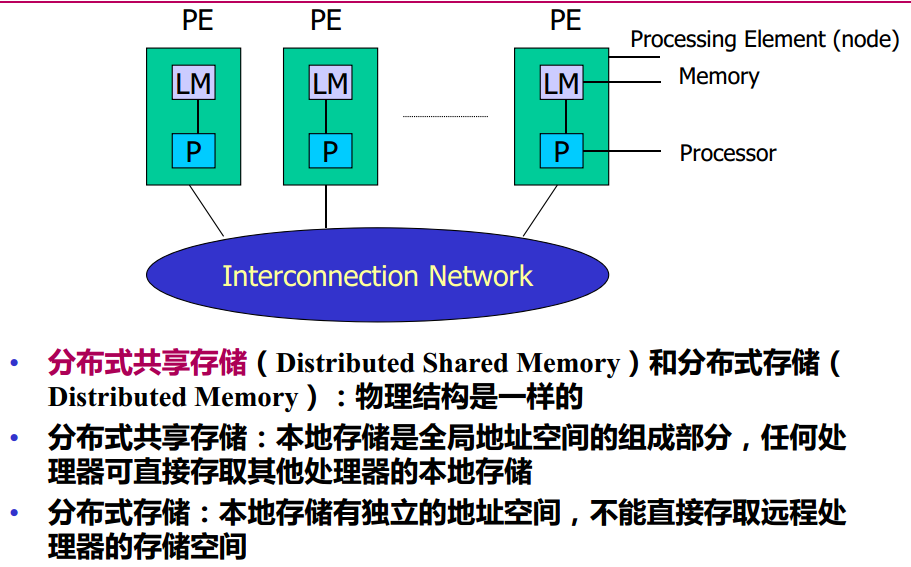
\includegraphics[scale = 0.3]{assets/ParallelComputing_c0e2d.png}
    \caption{DSM 分布式共享存储}
  \end{figure}
  注:\textbf{共享}体现在本地存储是否是全局地址空间的一部分

  \begin{figure}[H]
    \centering
    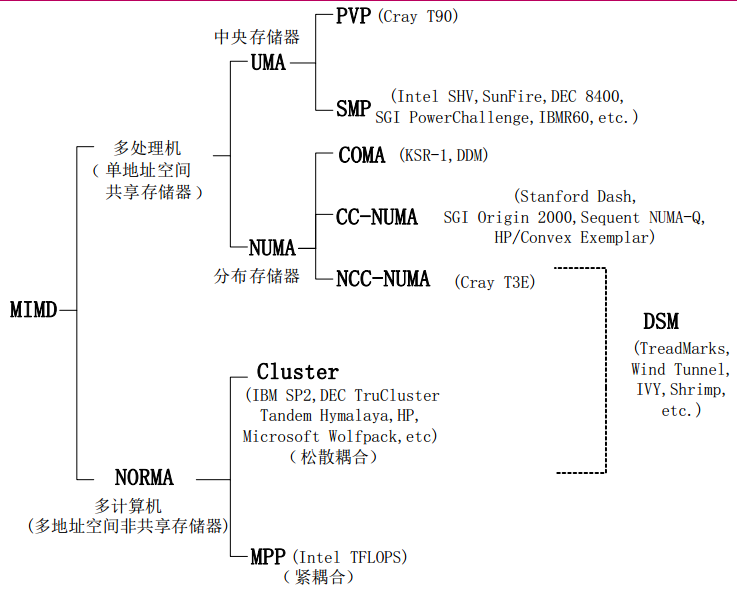
\includegraphics[scale = 0.3]{assets/ParallelComputing_f368c.png}
    \caption{并行系统的不同存储结构}
  \end{figure}

  \subsection{存储组织}
  为弥补CPU和主存之间的速度差异(平衡) , 需要多层存储的结构 ,各个层次间的访问速度和容量有差别

  \begin{figure}[H]
    \centering
    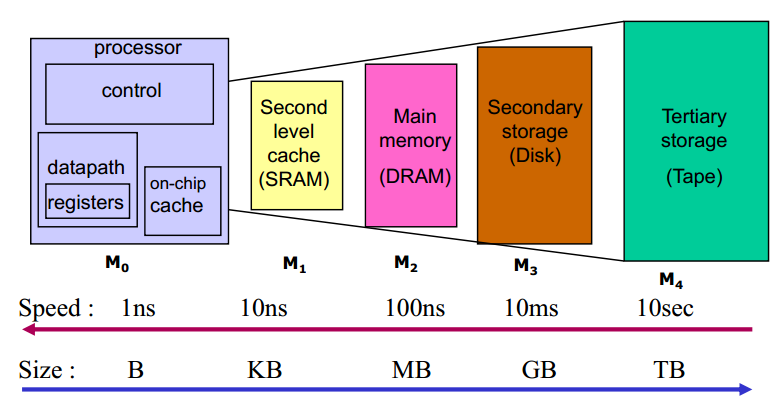
\includegraphics[scale = 0.3]{assets/ParallelComputing_fe648.png}
    \caption{存储层次结构}
  \end{figure}

  多层结构,可能会出现 \textbf{Cache不一致}的现象,主要原因为:
  \textbf{共享可写数据} 、 \textbf{多处理机的进程迁移}  、 \textbf{绕过Cache 的I/O 操作}

  解决缓存不一致的方法:
  \begin{itemize}
    \item 总线监听 : 所有处理器监听共享总线获知写操作, 以修改本地缓存\\
    有两种更新策略: \textbf{写无效}(写后缓存无效) 、 \textbf{写更新}(写后更新缓存) \\
    商业系统一般采用 写无效 , 以节省带宽
    \item 基于目录的协议 : 在主存中设置一个目录表 , 记录所有高速缓存的位置和状态 , 发送消息使得远程缓存无效或被更新\\
    每次写了之后更新主存的状态 , 当新的访问先检查状态, 如果是"脏"状态, 就从对应的处理器的缓存中更新内容到主存后再读取 ,并更新状态
  \end{itemize}

  \subsection{体系结构与访存模型}
  \begin{figure}[H]
    \centering
    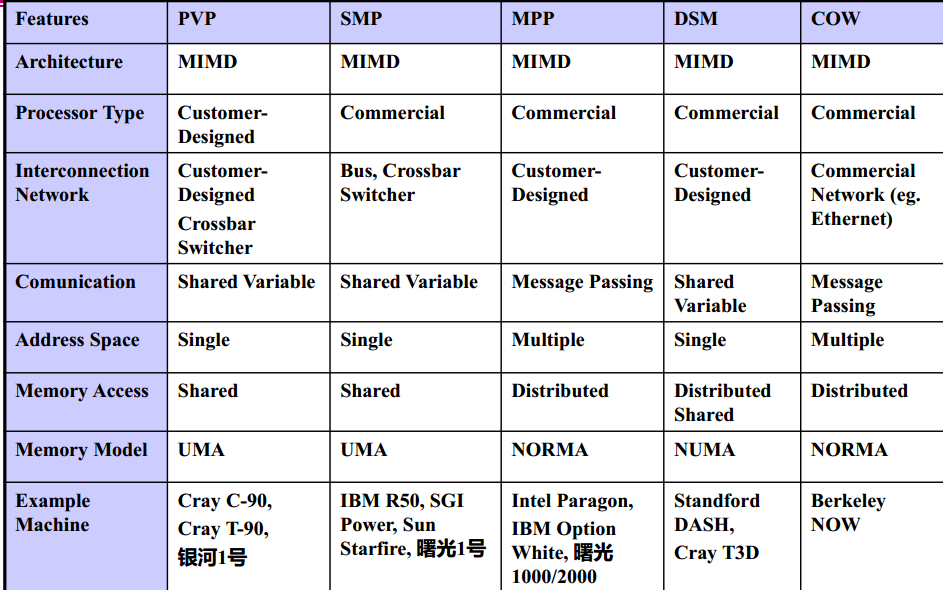
\includegraphics[scale = 0.3]{assets/ParallelComputing_cb9dc.png}
    \caption{体系结构与访存模型}
  \end{figure}

  SMP 、 MPP 、 DSM 、 COW 并行结构渐趋一致

  \section{并行计算性能评测}
  分类:
  \begin{itemize}
    \item 机器级的性能评测:CPU和存储器的某些基本性能指标 ; 并行和通信开销分析 ; 并行机的可用性与好用性 以及 机器成本 、价格 与性价比
    \item 算法级的性能评测:加速比 、效率 、 扩展性
    \item 程序级的性能评测 : 基准程序 (Benchmark)
  \end{itemize}

  \begin{figure}[H]
    \centering
    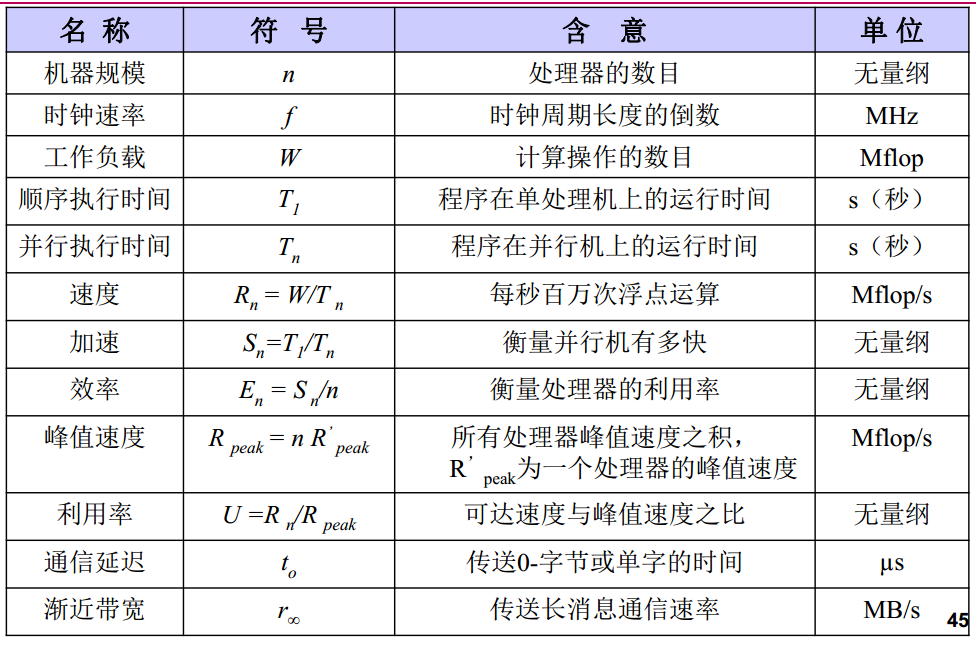
\includegraphics[scale = 0.3]{assets/ParallelComputing_d4d8f.png}
    \caption{并行机的性能}
  \end{figure}

  \subsection{加速比}
  \textbf{加速比} : 对于一个给定的应用 , 并行算法 或并行程序 相对于 串行算法 或 串行程序 的性能提高程度 ; 性能提高的通常表现为执行速度的加快
  \[S_p = \frac{\text{串行算法执行时间}}{\text{并行算法执行时间}}\]

  \textbf{并行效率} : 处理器的利用率
  \[\text{效率} =  \frac{\text{串行算法执行时间}}{\text{处理器数目}\times\text{并行算法执行时间}} = \frac{\text{加速比}}{\text{处理器数目}}\]

  \textbf{不同约束条件下的加速比}: \textbf{固定问题规模 PC} 、 \textbf{固定时间 TC} 、 \textbf{固定存储 MC}

  \textbf{符号定义:}
  \begin{itemize}
    \item $p$ : 处理器数目
    \item $W$ : 问题规模(计算负载 、 工作负载 、 给定问题的总计算量)
    \begin{itemize}
      \item $W_s$ : 应用程序中的串行分量
      \item $f$ : 串行分量比例 ($f = \frac{W_s}{W} , W_l = W_s + W_o$)
      \item $W_p$ : 应用程序中可并行化部分 , $1-f$为并行分量比例
      \item $W_s + W_p = W$
    \end{itemize}
    \item $T_l$:串行执行时间 , $T_p$ : 并行执行时间
    \item $S$ : 加速比
  \end{itemize}

  \begin{itemize}
    \item Amdahl 定律 : \textbf{固定不变的计算负载}  ,分布在多个处理器上; 增加处理器加快执行速度 ,从而达到加速的目的
    \begin{figure}[H]
      \centering
      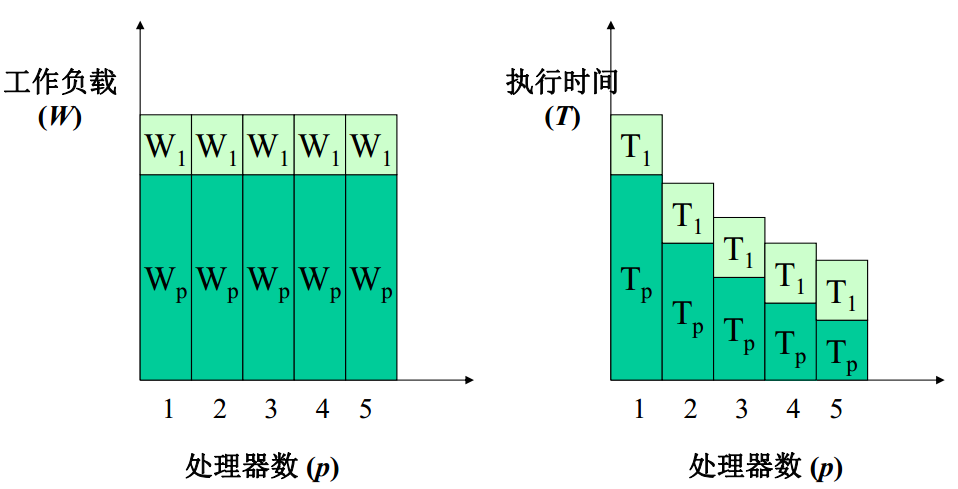
\includegraphics[scale = 0.3]{assets/ParallelComputing_f5c40.png}
      \caption{不同处理器数目下的问题规模 , 和对应的执行时间 ; 问题规模相同 , 串行时间不变 ,并行时间随着处理器数目增加而减少}
    \end{figure}
    Amdahl 定律 : 存在理论极限值 , 并行总计算量为$W_p$ 分配给 $p$个处理器
    \[S_{PC} = \frac{W_s + W_p}{W_s + W_p / p} = \frac{f + (1 - f)}{f + \frac{1 - f}{p}} = \frac{p}{1 + f(p - 1)} \to \frac{1}{f} \quad as\quad p \to \infty\]

    增强的Amdahl 定律 : 考虑开销 $W_o$(并行和通信的开销)
    \[S_{PC} = \frac{W_s + W_p}{W_s + W_p / p + W_o} = \frac{W}{fW + \frac{W(1 - f)}{p} + W_o} = \frac{p}{1 + f(p - 1) + W_0p / W} \to \frac{1}{f + \frac{W_o}{W}} \quad as \quad p \to \infty\]

    \item Gustafson 定律 : 在 \textbf{固定的时间} 内, 依靠增加处理器数目 期望能处理更多的数据
    \begin{figure}[H]
      \centering
      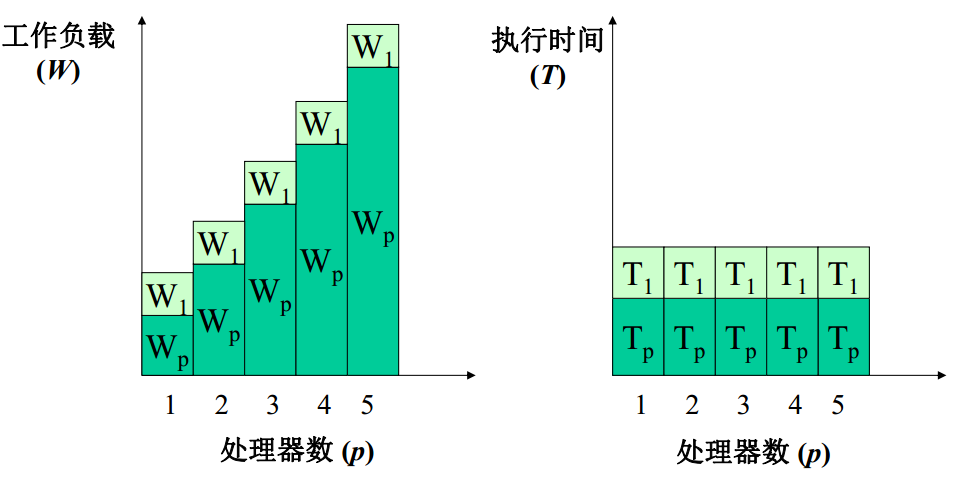
\includegraphics[scale = 0.3]{assets/ParallelComputing_4eeb1.png}
      \caption{不同处理器下, 每个处理器的时间相同, 以求能达到更多的计算总量}
    \end{figure}
    Gustafson 定律 : $p$个处理器 ,各自的计算量为$W_p$
    \[S_{TC} = \frac{W_S + pW_p}{W_s + pW_p / p} = \frac{W_s + pW_p}{W_s + W_p} \]
    \[S_{TC} = f + p(1 - f) = p + f(1 - p) = p - f(p - 1)\]
     (这里定义的$W_p$是的那个处理器的工作量, $f = \frac{W_s}{W_s + W_p} \neq \frac{W_s}{W}$)

     考虑开销:
     \[S_{TC} =  \frac{W_s + pW_p}{W_s + W_p + W_o} = \frac{f + p(1 - f)}{1 + W_o / W} \]

    \item Sun Ni 定律 : 只要存储空间许可 ,应尽量增大问题 即 \textbf{固定存储}(尽可能利用完全部存储)时能发挥多大的性能\\
    假定在单个节点上使用了全部存储容量M并在相应于W的时间内求解之 , 此时工作负载:
    \[W = fW + (1 - f)W\]
    在p个节点的并行系统上 , 能求解较大的问题是因为存储容量可增加到$pM$(一个节点为$M$) , 令因子$G(p)$表示 \textbf{存储容量增加到p倍时,并行计算负载的增加量} ,则
    \[W = fW + (1 - f)G(p)W\]
    \begin{figure}[H]
      \centering
      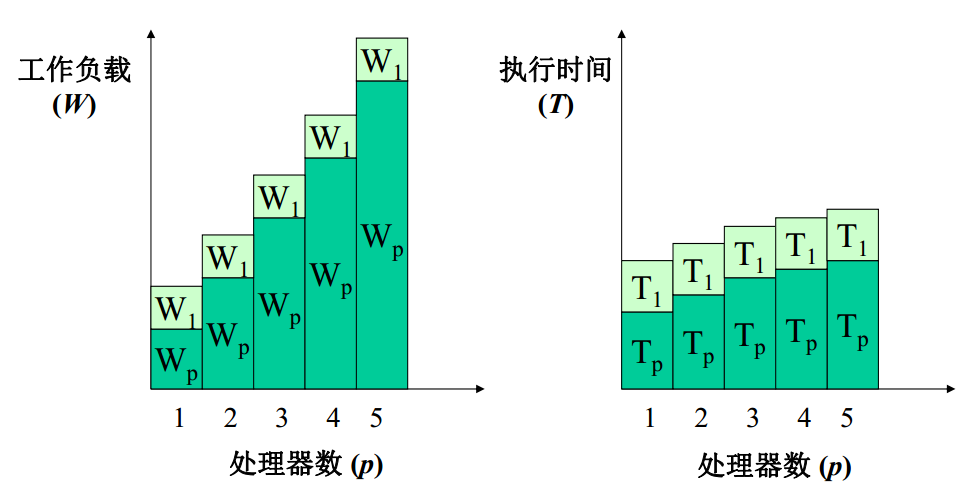
\includegraphics[scale = 0.3]{assets/ParallelComputing_8cabd.png}
      \caption{并行时间和并行负载都增加}
    \end{figure}

    Sun Ni 定律: 存储受限的加速公式
    \[S_{MC} = \frac{fW + (1 - f)G(p)W}{fW + (1  -f)G(p)W / p} = \frac{f +(1 - f)G(p)}{f + (1 - f)G(p) / p}\]

    考虑并行开销:
    \[S_{MC} = \frac{fW + (1 - f)G(p)W}{fW + (1  -f)G(p)W / p + W_o} = \frac{f +(1 - f)G(p)}{f + (1 - f)G(p) / p + W_o / W}\]

    G(p) = 1 时 , 就是 Amdahl 加速定律\\
    G(p) = p 时 , 就是 Gustafson 加速定律\\
    当$G(p) > p$ 时,相应于计算机负载比存储要求增加得快

  \end{itemize}

  \textbf{影响加速比的因素} :
  \begin{itemize}
    \item 求解问题中的串行分量
    \item 并行处理所引起的额外开销(通信 、 等待 、 竞争 、 冗余 操作 、 同步)
    \item 加大的处理器数超过了算法中的并发度
  \end{itemize}

  \textbf{增加问题规模有利于提高加速的因素}:
  \begin{itemize}
    \item 较大的问题规模可提供较高的并发度
    \item 额外开销的增加可能慢于有效计算的增加
    \item 算法中的串行分量比例不是固定不变的(串行部分所占比例随着问题规模的增大而缩小)
  \end{itemize}

  \textbf{绝对加速} : 最佳并行算法与串行算法(科学研究)

  \textbf{相对加速} : 同一算法 在单机和并行机的运行时间(工程应用)

  \subsection{可扩展性}

  \textbf{可扩展性} : 当系统的问题规模增大时, 可维持相同性能的能力 , 即指应用、算法和结构能否充分利用不断增长的处理器的能力 (性能、系统规模、数据规模的综合测度)

  增加系统规模(处理器数目)会增大额外的开销和降低处理器利用率 , 所以对于一个特定的并行系统(算法或程序) , 他们能否有效利用不断增肌的处理器的能力应是受限的 , 而度量这种能力就是 \textbf{可扩方性} 这一指标

  加速比:
  \[S = \frac{T_e}{T_p} = \frac{T_e}{\frac{T_e + T_o}{p}} = \frac{p}{1 + \frac{T_o}{T_e}} = \frac{p}{1 + \frac{W_o}{W}}\]

  效率:
  \[E = \frac{S}{P}=\frac{1}{1 + \frac{T_o}{T_e}} = \frac{1}{1 + \frac{W_o}{W}}\]
  当问题规模$W$保持不变 , 处理器数目$p$增加, 开销$T_o$增大,效率$E$下降 , 为了保持$E$不变, 需要增大$W$

  \begin{itemize}
    \item 等效率度量标准
    \item 等速度度量标准
    \item 平均延迟度量标准
  \end{itemize}

  \begin{figure}[H]
    \centering
    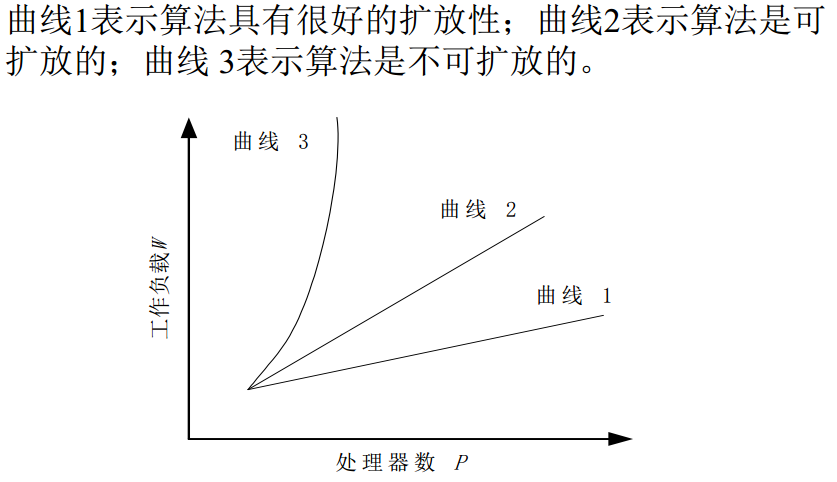
\includegraphics[scale = 0.3]{assets/ParallelComputing_c2124.png}
  \end{figure}

  \section{并行算法模型}
  \textbf{成本最优性} : 若$c(n)$等于在最坏的情况下串行算法所需要的时间 , 则并行算法是最优的(并行算法的时间和等于串行算法最差时间)
    \begin{itemize}
      \item 运行时间$t(n)$
      \item 处理器数目$p(n)$
      \item 成本 $c(n) = t(n) \times p(n)$
      \item 问题规模 $n$
    \end{itemize}

  \subsection{PRAM模型}
  \textbf{PRAM模型}: 由 Fortune 和 Wyllie 1978年提出 ,又称 \textbf{SIMD-SM模型}

  \begin{itemize}
    \item 有一个集中的共享UC能出其和一个指令控制器 , 通过共享存储(SM) 的 Read / Write 交换数据 , 隐式同步计算
    \item 在一个时钟周期内,每个处理器执行一条指令 , 可完成3个操作 : 从存储器取出一个操作数 ,完成一个算数 、逻辑运算 , 将结果存回存储器
  \end{itemize}
  \begin{figure}[H]
    \centering
    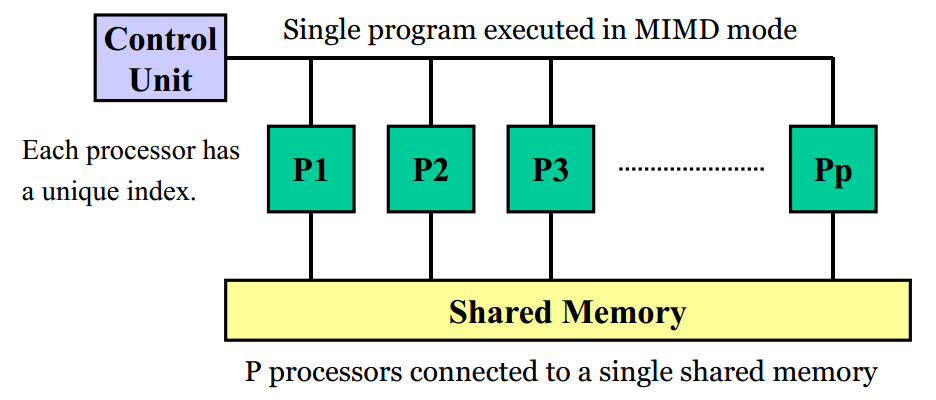
\includegraphics[scale = 0.3]{assets/ParallelComputing_4dc7b.png}
    \caption{PRAM 结构图}
  \end{figure}

  \textbf{PRAM模型的特点}:
  \begin{itemize}
    \item 全局共享存储 , 单一地址空间
    \item 同步 、 通信 和并行化的开销为 0
  \end{itemize}

  \textbf{PRAM模型的优点:}
  \begin{itemize}
    \item 简单 : 适合合并算法表示和复杂性分析 , 易于使用\\
    PRAM模型特别适合并行算法的表达、分析 、比较
    \item 易于扩展 : 隐藏了并行机的通讯 、同步等细节\\
    根据需要 , 可以在 PRAM模型中加入 诸如同步 、通信等需要考虑的内容
  \end{itemize}

  \textbf{PRAM模型的缺点}:
  \begin{itemize}
    \item 模型中使用了一个全局共享存储器 , 不适合 分布存储结构的并行机
    \item PRAM 模型是同步的, 不能反映现实中很多系统的异步性
    \item 不适合MIMD并行机, 忽略了SM的竞争、通信延迟等因素
  \end{itemize}

  \textbf{存储数据的存储模型:}
  \begin{itemize}
    \item CRCW : 并发读 并发写 , 冲突解决模式:
    \begin{itemize}
      \item 公共并发读写 Common CRCW : 仅允许写入相同数据
      \item 优先并发读写 Priority CRCW : 仅允许优先级最高的处理器写入
      \item 任意并发读写 Arbitrary CRCW : 允许任意处理器自由写入
    \end{itemize}
    \item CREW : 并发读 互斥写
    \item EREW : 互斥读 互斥写
  \end{itemize}

  \textbf{其他PRAM}:
  \begin{itemize}
    \item 分相 PRAM : 一个异步的PRAM 模型 , 各个处理器异步地执行局部程序 ,每个局部陈旭的最后一条语句是同步障指令
    \item 本地存储 PRAM LPRAM : 考虑本地存储和远程存储的开销不同
    \item 块PRAM BPRAM : LPRAM + 通信开销
  \end{itemize}

  \subsection{BSP模型}

  \textbf{BSP模型} Bulk Synchronous Parallel  : 块同步模型 , 是一种异步 \textbf{MDMD - DM} 分布式存储 模型 , 支持消息传递系统 , 块内异步执行 , 块间显示同步

  \textbf{BSP模型的3个组成部分}:
  \begin{itemize}
    \item 节点 : 处理器 , 本地存储
    \item 通信网络 : 点到点 , 消息传递
    \item 同步障 : 同步机制
  \end{itemize}

  \begin{figure}[H]
    \centering
    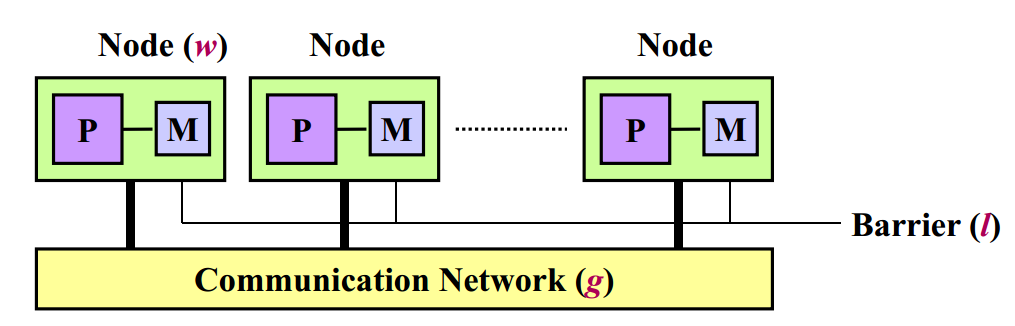
\includegraphics[scale = 0.3]{assets/ParallelComputing_d4198.png}
    \caption{BSP 图例}
  \end{figure}

  \textbf{超步} : BSP 计算过程由若干个超级步组成
  \begin{figure}[H]
    \centering
    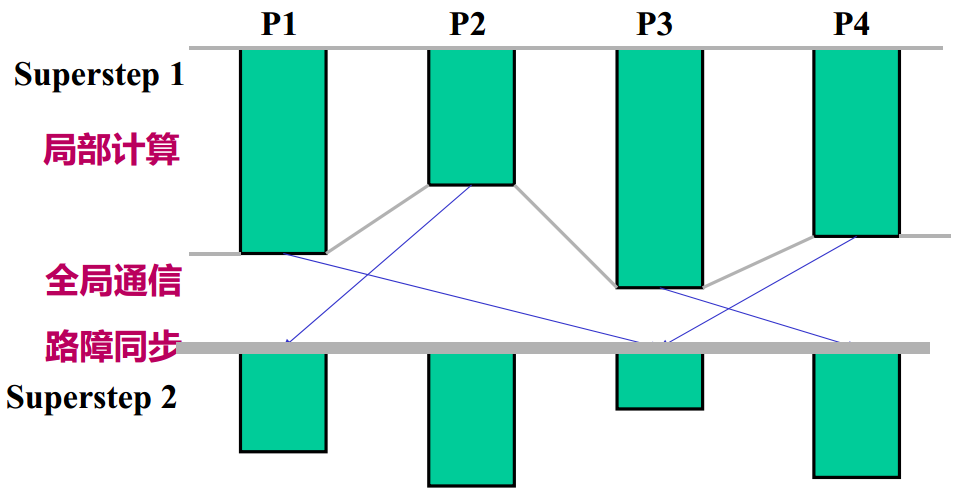
\includegraphics[scale = 0.3]{assets/ParallelComputing_bf7df.png}
    \caption{超步}
  \end{figure}

  \textbf{模型参数}:
  \begin{itemize}
    \item $w$ : 计算参数 \\
    每个超步内最大的计算时间 , 计算操作最多为$w$个时钟周期
    \item $g$ : 带宽参数 $g = \frac{1}{bandwidth}$ , 单位消息所需的通信时钟 - 网络带宽的倒数 \\
    关系因子 h : 每个节点至多发送和接受h个消息 , 通信操作最多为 $gh$个时钟周期
    \item $l$ : 同步障参数 , 同步障操作最多为$l$个时钟周期
  \end{itemize}

  BSP 模型的时间复杂度:
  \begin{itemize}
    \item Valiant 公式 : 计算与通信 重叠
    \[max\{w,  gh , l\}\]
    \item McCpll 重写后的公式 :
    \[w + gh + l\]
  \end{itemize}

  \textbf{例子 : 点积}$2N / P + \log p(g + l  +1)$($\log p$次求和(通信)和同步)
  \begin{figure}[H]
    \centering
    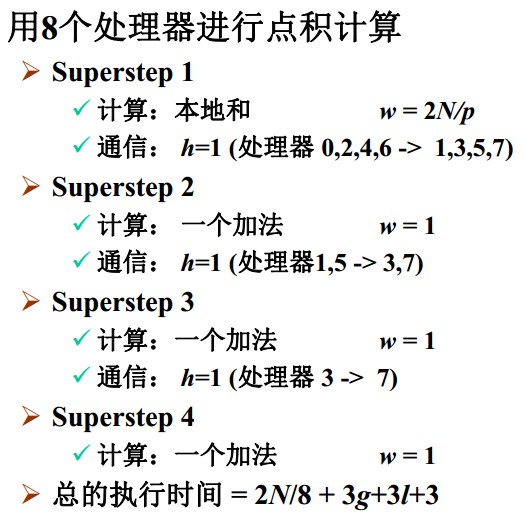
\includegraphics[scale = 0.3]{assets/ParallelComputing_bbb01.png}
    \caption{BSP 点积 :就是每个阶段的最大时间 和}
  \end{figure}

  对比 \textbf{PRAM}模型: $LN / p + \log p$(不考虑同步和通信)

  \textbf{BSP 模型 的优点}:
  \begin{itemize}
    \item BSP模型视图为软件和硬件之间建立起一座类似冯诺依曼机的桥梁 , 因此 , BSP模型也常叫 \textbf{桥模型}
    \item 将处理器和路由器分开 ,\textbf{强调计算任何和通信任务的分开} , 而路由器仅仅完成点到点的消息传递 , 不提供组合 、 复制和广播等功能 , 这样做既掩盖具体的互连网络拓扑,又简化了通信协议
  \end{itemize}

  \textbf{BSP 模型的缺点} :
  \begin{itemize}
    \item 需要显示同步 ,编程效率不高
    \item BSP模型中的全局障碍同步假定是用特殊硬件支持的, 这在很多并行机中可能没有相应的硬件
  \end{itemize}


  \subsection{logP模型}
  \textbf{log P 模型} : 有 Culler 1993年提出 ,是一种分布存储的 、点到点通信的多处理机模型 ,其中通讯由一组参数描述 ,实行隐式同步

  \textbf{模型参数}:
  \begin{itemize}
    \item $L$ : 网络时延
    \item $o$ : 通信开销
    \item $g$ : $gap \quad \frac{1}{bandwidth}$ , 经过$g$才能再次发送
    \item $P$ : $\# processors$
    注: $L$和$g$反映了通讯网络的容量
  \end{itemize}

  \begin{figure}[H]
    \centering
    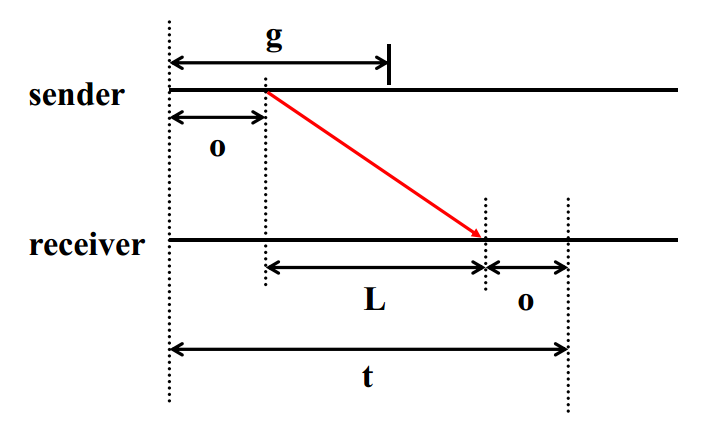
\includegraphics[scale = 0.3]{assets/ParallelComputing_2f864.png}
    \caption{Log P 图例}
  \end{figure}

  \textbf{Log P 模型的优点}:
  \begin{itemize}
    \item 异步模型 ,没有同步障
    \item 捕捉了并行计算机的通讯瓶颈
    \item 通信由一组参数描述 ,但并不涉及具体的网络结构 ,隐藏了并行机的网络拓扑、路由 、协议
    \item 可以应用到共享存储 、 消息传递 、 数据并行 的编程模型中
  \end{itemize}

  \textbf{Log P 模型的缺点}:
  \begin{itemize}
    \item 难以进行描述 、设计 和分析
    \item 对网络中的通信模式描述得不够深入 \\
    如重发消息可能占满带宽 、中间路由器缓存饱和 等未加描述
    \item Log P 模型主要适用于消息传递算法设计 ,对于共享存储模式 ,则简单地认为远程读取操作相当于两次消息传递 ,未考虑流水线预取技术 、 Cache引起的数据不一致性 以及 Cache 命中率对计算的影响
  \end{itemize}

  \textbf{BSP 和 Log P的比较}
  \begin{itemize}
    \item BSP分为 : BSP 块同步  , BSP 子集同步 , BSP 进程对同步\\
    其中 , BSP 进程对同步 = Log P
    \item BSP可以常数因子模拟 Log P , Log P 可以对数因子模拟 BSP
    \item BSP提供了更方便的的程序设计环境, Log P 更好地利用了机器资源
    \item BSP 似乎更方便、简单 和 符合结构化编程
  \end{itemize}

  \begin{figure}[H]
    \centering
    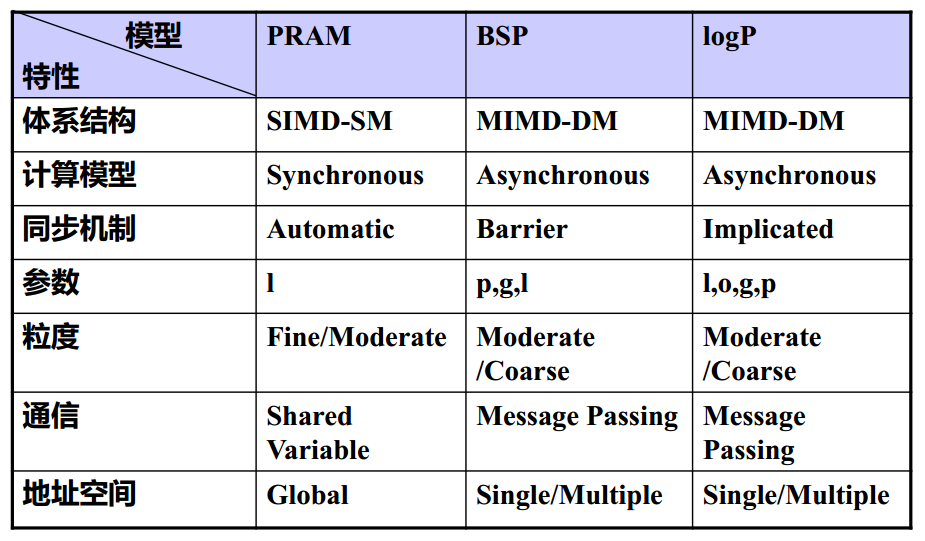
\includegraphics[scale = 0.3]{assets/ParallelComputing_e3d13.png}
    \caption{三种模型的对比}
  \end{figure}

  \subsection{并行算法的一般设计方法}
  \begin{itemize}
    \item 串行算法直接并行化
    \item 从问题描述开始设计并行算法
    \item 借用已有的算法求解新问题
  \end{itemize}

  \section{并行算法设计技术}
  \subsection{平衡树方法}
  叶节点为输入,中间节点处理,由叶向跟逐层并行处理
  \begin{figure}[H]
    \centering
    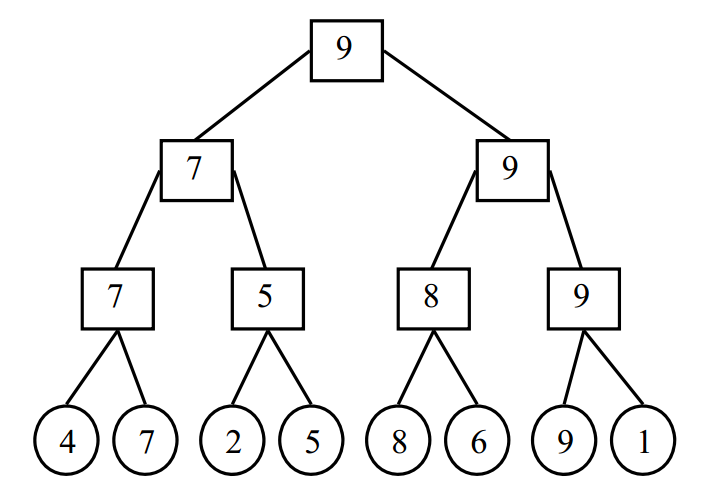
\includegraphics[scale = 0.3]{assets/ParallelComputing_32d59.png}
    \caption{求最大值}
  \end{figure}

  \begin{figure}[H]
    \centering
    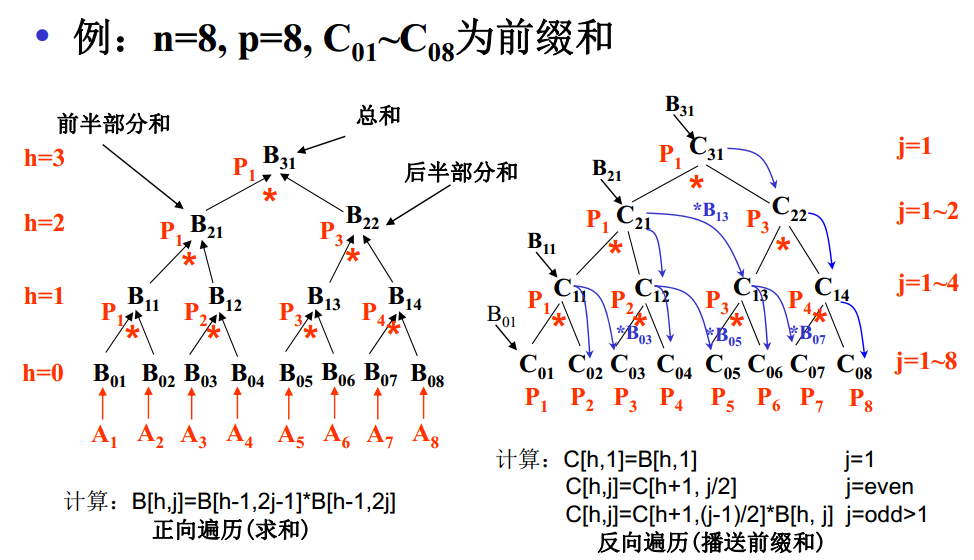
\includegraphics[scale = 0.3]{assets/ParallelComputing_2f254.png}
    \caption{求前缀和 : 分为两个过程 (1)正向遍历求和(从叶子向跟逐层并行) (2)反向遍历播送前缀和(从根向叶子 ,逐层并行)}
  \end{figure}

  \begin{figure}[H]
    \centering
    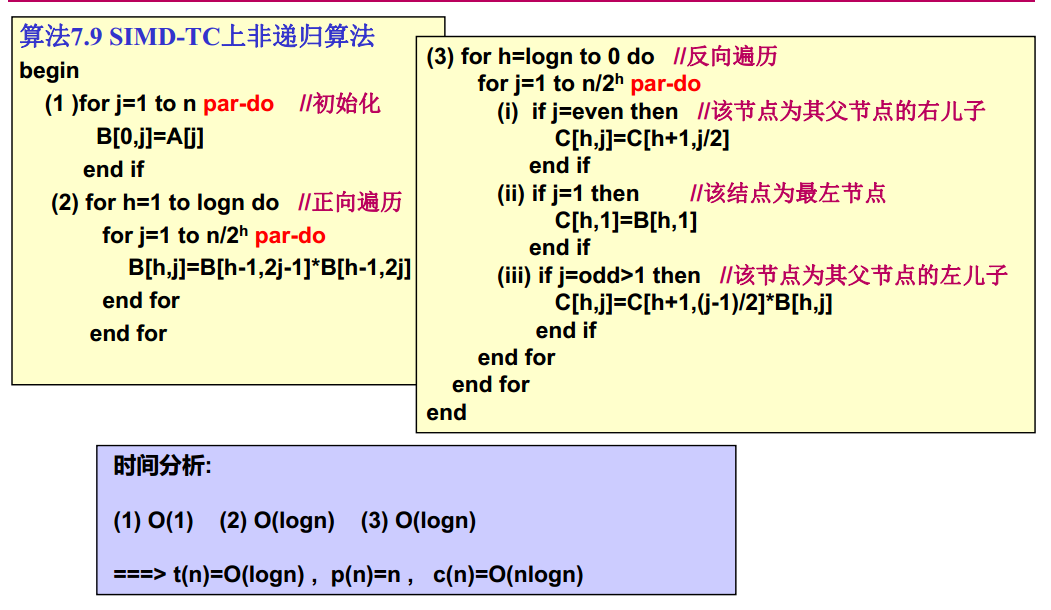
\includegraphics[scale = 0.3]{assets/ParallelComputing_903f7.png}
    \caption{求前缀积并行算法(这里是积哦)}
  \end{figure}

  \subsection{倍增技术}
  \textbf{倍增技术} : 又称 \textbf{指针跳跃技术} , 特别适合处理链表或有向树之类的数据结构 , 当递归调用时 ,所要处理数据之间的距离逐步加倍 ,经过k步之后即可完成距离为$2^k$的所有数据的计算

  比如 : \textbf{表序问题} , \textbf{求森林的根}

  \begin{itemize}
    \item 表序问题 : n个元素的列表 L ,求出每个元素在 L中的次第号 (秩 或 位序 或 rank(k) ) , rank(k) 可以视为元素k至表位的距离 , 且每个元素分配一个处理器
    \begin{figure}[H]
      \centering
      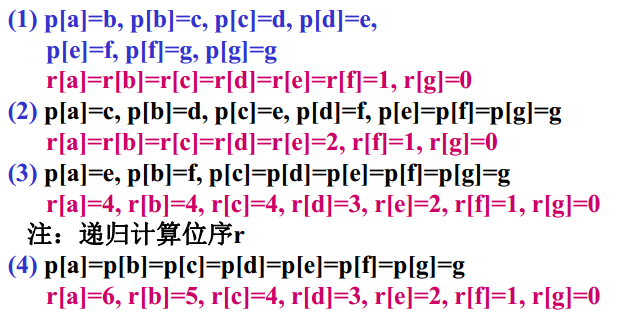
\includegraphics[scale = 0.3]{assets/ParallelComputing_dd12c.png}
      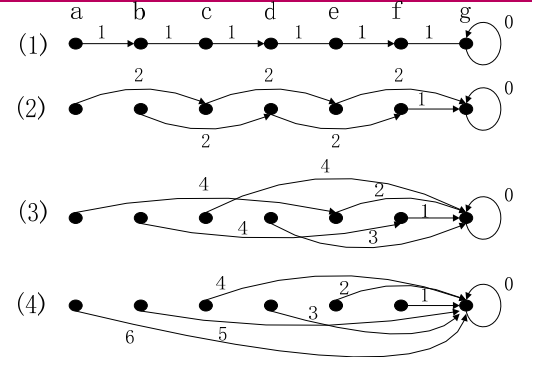
\includegraphics[scale = 0.3]{assets/ParallelComputing_fc17e.png}
      \caption{表序问题实例}
    \end{figure}
    \begin{figure}[H]
      \centering
      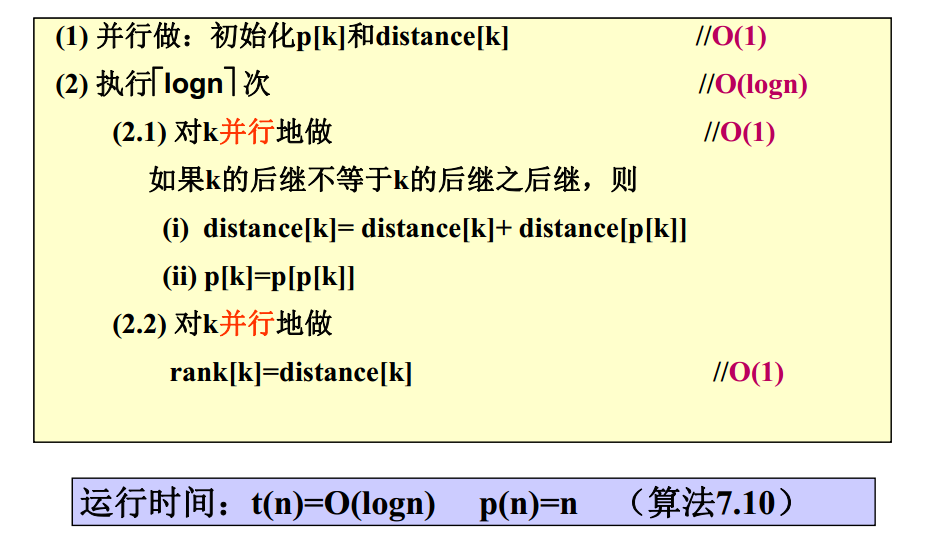
\includegraphics[scale = 0.3]{assets/ParallelComputing_5f843.png}
      \caption{求元素表序算法}
    \end{figure}
    \item 求森林的根 : 一组有向树F种 , 如果(i,j) 是F中的一条弧 , 则p[i] = j ,(j是i的双亲) ; 若i为根 ,则p[i] = i, 求每个节点j的树根 s[j]\\
    类似并查集的路径压缩\\
    \begin{figure}[H]
      \centering
      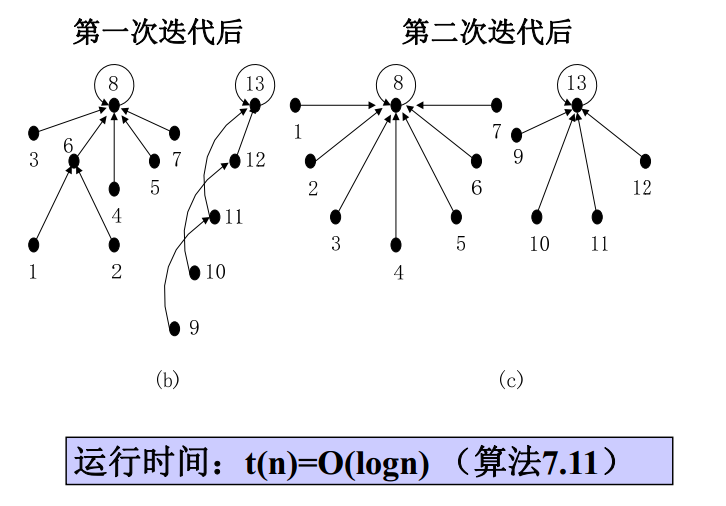
\includegraphics[scale = 0.3]{assets/ParallelComputing_8ca98.png}
      \caption{求森林的根 实例}
    \end{figure}
  \end{itemize}
  \subsection{分治策略}
  \textbf{求解步骤}
  \begin{itemize}
    \item 将输入划分为若干个规模相等的子问题
    \item \textbf{并行地}递归求解这些子问题
    \item \textbf{并行地}归并子问题的解称为原问题的解
  \end{itemize}

  \begin{figure}[H]
    \centering
    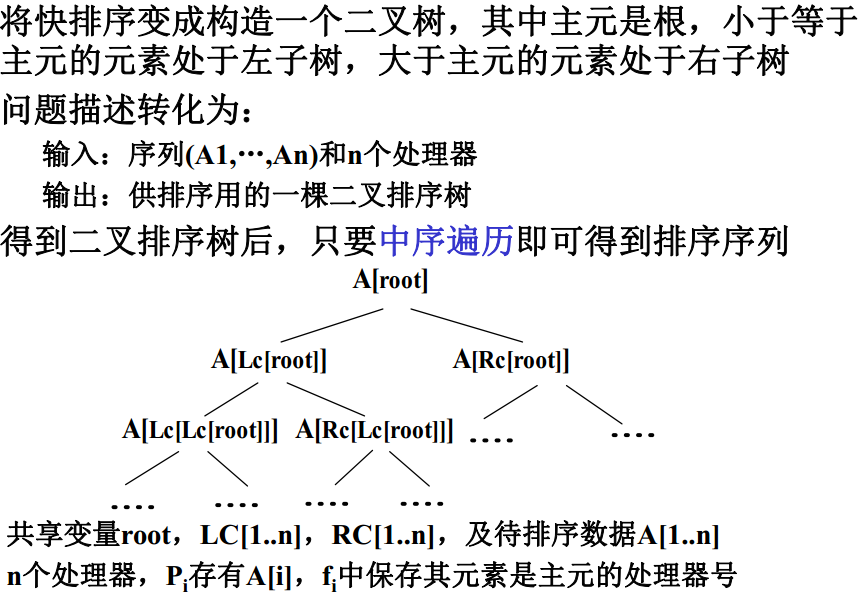
\includegraphics[scale = 0.3]{assets/ParallelComputing_1d815.png}
    \includegraphics[scale = 0.3]{assets/ParallelComputing_e897a.png}
    \caption{并行快速排序算法}
  \end{figure}

  \begin{itemize}
    \item 同时写
    \item 从根节点开始构造二叉树
    \item 每个节点为快排的支点
    \item 每个节点均写入root,最终留在root中的作为支点
    \item 其他节点与父节点比较,确定左子树还是右子树
    \item 每个子树重复这个步骤
    \item 中序遍历得到排序结果
  \end{itemize}

  {\sout{写入root的时候是随意写的,而读取root的时候未必能保证root已经写完了,如果没写完,那么读取的节点就不一定是根节点呀} , 有同步障,问题?不存在的}

  \subsection{划分原理}
  \textbf{划分原理设计思想:}将原问题划分为p个独立的规模几乎相等的子问题 , p台处理机并行地求解各个子问题

  \textbf{划分的重点在于}:子问题易解 , 组合成原问题的解方便

  \subsubsection{均匀划分}
  方法:分组长度取$\frac{n}{p}$
  \begin{figure}[H]
    \centering
    \includegraphics[scale = 0.3]{assets/ParallelComputing_c0fc1.png}
    \caption{均匀划分}
  \end{figure}

  \begin{figure}[H]
    \centering
    \includegraphics[scale = 0.3]{assets/ParallelComputing_7763b.png}
    \caption{PSRS 排序算法}
  \end{figure}

  \subsubsection{方根划分}
  方法:分组长度取$\sqrt{n}$
  \begin{figure}[H]
    \centering
    \includegraphics[scale = 0.3]{assets/ParallelComputing_aff77.png}
    \caption{方根划分}
  \end{figure}

  \begin{figure}[H]
    \centering
    \includegraphics[scale = 0.3]{assets/ParallelComputing_a3e6a.png}
    \caption{Valiant 归并排序算法}
  \end{figure}

  \subsubsection{对数划分}
方法:分组长度取$\log{n}$
\begin{figure}[H]
  \centering
  \includegraphics[scale = 0.3]{assets/ParallelComputing_618be.png}
  \caption{对数划分}
\end{figure}

  \subsubsection{功能划分}

  \begin{figure}[H]
    \centering
    \includegraphics[scale = 0.3]{assets/ParallelComputing_01061.png}
    \caption{功能划分技术 - n个求前m个最小 : 分成多组 ,每组m个, 每两组合并成一组(大小为m),直到剩下一个}
  \end{figure}

  \begin{figure}[H]
    \centering
    \includegraphics[scale = 0.3]{assets/ParallelComputing_a7ba0.png}
    \caption{功能划分 - n个求前m个最小}
  \end{figure}


  \subsection{流水线}
  \textbf{流水线 设计思想}:将算法流程划分成p个前后衔接的任务片段 ,每个任务片段的输出作为下一个任务片段的输入 , 所有任务片段按相同的速度产生出结果

  \begin{figure}[H]
    \centering
    \includegraphics[scale = 0.3]{assets/ParallelComputing_a5d0f.png}
    \caption{DFT}
  \end{figure}

  \begin{figure}[H]
    \centering
    \includegraphics[scale = 0.3]{assets/ParallelComputing_1adbb.png}
    \includegraphics[scale = 0.3]{assets/ParallelComputing_6426f.png}
    \caption{5-point DFT的计算}
  \end{figure}

  \section{并行算法一般设计过程}
  并行算法一般设计过程:划分,通信,组合,映射(PCAM)
  \begin{itemize}
    \item 划分 Partition : 分解成小的任务 ,开拓并发性\\
    分为 : \textbf{域划分(数据划分)} 、 \textbf{功能划分}\\
    要求划分之后各任务的数据不相交
    \begin{figure}[H]
      \centering
      \includegraphics[scale = 0.3]{assets/ParallelComputing_64f1a.png}
      \caption{域分解}
    \end{figure}
    \item 通信 Communication : 确定诸任务间的数据交换 ,检测划分的合理性
    4种通信模式: \textbf{局部/全局通信} 、 \textbf{结构化 / 非结构化通信}
    、 \textbf{静态/动态通信} 、 \textbf{同步 /异步 通信}

    \item 组合 Agglomeration : 依据任务的局限性, 组合成更大的任务
    \begin{figure}[H]
      \centering
      \includegraphics[scale = 0.3]{assets/ParallelComputing_e3e03.png}
      \caption{组合例子}
    \end{figure}

    \textbf{表面-容积效应}: 通信量与任务子集表面积成正比 , 计算量与任务子集的体积成正比 ; 增加重复计算可以减少通信量

    \item 映射 Mappnig : 将每个任务分配到处理器上 , 提高算法的性能\\
    目标是最小化总的执行时间(保持负载平衡)
  \end{itemize}

  \begin{figure}[H]
    \centering
    \includegraphics[scale = 0.3]{assets/ParallelComputing_af04f.png}
    \caption{PCAM 设计过程}
  \end{figure}

\textbf{划分判据}
\begin{itemize}
  \item 划分是否具有灵活性?
  \item 划分是否避免了冗余计算和存储?
  \item 划分任务尺寸是否大致相当?
  \item 任务数与问题尺寸是否成比例?
  \item 是否能分解是种更深层次的分解,合理?
\end{itemize}


\textbf{通信判据}
\begin{itemize}
  \item 所有任务是否执行大致相当的通信?
  \item 是否尽可能的局部通信?
  \item 通信操作是否能并行执行?
  \item 同步任务的计算能否并行执行?
\end{itemize}

\textbf{组合判据}
\begin{itemize}
  \item 增加粒度是否减少了通信成本?
  \item 重复计算是否已权衡了其得益?
  \item 是否保持了灵活性和可扩展性?
  \item 组合的任务数是否与问题尺寸成比例?
  \item 是否保持了类似的计算和通信?
  \item 有没有减少并行执行的机会?
\end{itemize}
\textbf{映射判据}
\begin{itemize}
  \item 采用集中式负载平衡方案,是否存在通信瓶颈?
  \item 采用动态负载平衡方案,调度策略的成本如何?
\end{itemize}

\section{并行程序设计基础}
\subsection{Cannons 矩阵乘法}
\begin{figure}[H]
  \centering
  \includegraphics[scale = 0.3]{assets/ParallelComputing_2c3d9.png}
  $\to$
  \includegraphics[scale = 0.3]{assets/ParallelComputing_84070.png}
  \caption{每个三角代表一块矩阵块, 相同颜色表示可以相乘; 块$A_{ij}$向左循环移动$i$步 , 块$B_{ij}$向上循环移动$j$步}
\end{figure}

\begin{figure}[H]
  \centering
  \includegraphics[scale = 0.3]{assets/ParallelComputing_e6eb5.png}
  \caption{Cannon 算法描述}
\end{figure}
\begin{figure}[H]
  \centering
  \includegraphics[scale = 0.3]{assets/ParallelComputing_962bf.png}
  \caption{Cannon伪代码}
\end{figure}
\begin{figure}[H]
  \centering
  \includegraphics[scale = 0.3]{assets/ParallelComputing_df3c9.png}
  \caption{Cannon 复杂度分析}
\end{figure}

\subsection{DNS 矩阵乘法}
\begin{figure}[H]
  \centering
  \includegraphics[scale = 0.3]{assets/ParallelComputing_a5e25.png}
  \caption{矩阵乘法示意}
\end{figure}

\begin{figure}[H]
  \centering
  \includegraphics[scale = 0.3]{assets/ParallelComputing_e8daa.png}
  \caption{DNS 矩阵乘法思路}
\end{figure}

\begin{figure}[H]
  \centering
  \includegraphics[scale = 0.3]{assets/ParallelComputing_86ce4.png}
  \caption{DNS 矩阵分块}
\end{figure}

\begin{figure}[H]
  \centering
  \includegraphics[scale = 0.3]{assets/ParallelComputing_04086.png}
  \caption{DNS 矩阵乘法 算法描述}
\end{figure}

\begin{figure}[H]
  \centering
  \includegraphics[scale = 0.3]{assets/ParallelComputing_8c711.png}
  \includegraphics[scale = 0.3]{assets/ParallelComputing_23b58.png}
  \caption{DNS 矩阵乘法 伪代码}
\end{figure}

\section{并行编程风范}
\subsection{相并行}
相并行 :一组超步 ; 步内各自计算 ; 步间通信、同步 ; BSP ; 方便差错和性能分析 ; 计算和通信不能重叠

\begin{figure}[H]
  \centering
  \includegraphics[scale = 0.3]{assets/ParallelComputing_5c10e.png}
  \caption{相并行}
\end{figure}

\subsection{分治并行}
分治并行 : 父进程把负载分割指派给子进程 ; 递归 ; 重点在于归并 ;难以负载平衡
\begin{figure}[H]
  \centering
  \includegraphics[scale = 0.3]{assets/ParallelComputing_d2aa6.png}
  \caption{分治并行}
\end{figure}

\subsection{流水线并行}
流水线并行 : 一组进程 ; 流水线作业
\begin{figure}[H]
  \centering
  \includegraphics[scale = 0.3]{assets/ParallelComputing_34d57.png}
  \caption{流水线并行}
\end{figure}

\subsection{主从并行}
主进程 : 串行 、 协调任务

子进程 : 计算子任务

主从并行: 与相并行易结合 , 主进程易成为瓶颈(有点类似分治 ,但这里不要求是划分子任务)

\begin{figure}[H]
  \centering
  \includegraphics[scale = 0.3]{assets/ParallelComputing_703c4.png}
  \caption{主从并行}
\end{figure}

\subsection{工作池并行}
工作池并行 : 进程从池中去任务执行 ,可产生新任务放回池中 ,初始为一件工作 ,直到任务池为空 ; 易负载平衡 , 存在临界区问题

\begin{figure}[H]
  \centering
  \includegraphics[scale = 0.3]{assets/ParallelComputing_12327.png}
  \caption{工作池并行}
\end{figure}

\begin{figure}[H]
  \centering
  \includegraphics[scale = 0.3]{assets/ParallelComputing_b2389.png}
  \includegraphics[scale = 0.3]{assets/ParallelComputing_d61b4.png}
  \includegraphics[scale = 0.3]{assets/ParallelComputing_d02ee.png}
  \includegraphics[scale = 0.3]{assets/ParallelComputing_1c40a.png}
  \includegraphics[scale = 0.3]{assets/ParallelComputing_66d2d.png}
  \caption{计算点积}
\end{figure}

\section{并行程序设计的基本问题}
\subsection{进程的同构性}
\begin{itemize}
  \item SIMD : 所有进程在同一时间执行相同的指令
  \item MIMD : 各个进程在同一时间可以执行不同的指令
  \begin{itemize}
    \item SPMD Single Program Multiple Data : 各个进程是同构的,多个进程对不同的数据执行相同的代码(一般是数据并行的同义语, 常对应并行循环 , 数据并行结构 , 单代码)
    \item MPMD Multiple Program Multiple Data : 各个进程是异构的 , 多个进程执行不同的代码 (一般是任务并行 , 功能并行 或 控制并行的同义语 , 常对应 并行块 ,多代码)
  \end{itemize}
\end{itemize}

\subsection{静态和动态并行性}
\begin{itemize}
  \item 静态并行性 : 程序的结构以及进程的个数在运行之前就可确定
  \item 动态并行性 : 否则就认为程序具有动态并行性, 即意味着程序要在运行时创建和终止
\end{itemize}

\subsection{进程分配}
\begin{figure}[H]
  \centering
  \includegraphics[scale = 0.3]{assets/ParallelComputing_424f5.png}
\end{figure}

\subsection{并行粒度}
并行度 : 同时执行的分进程数

并行粒度 : 两次并行 或 交互操作之间所执行的计算负载
\begin{itemize}
  \item 指令级并行
  \item 块级(数据级)并行
  \item 进程级(控制级)并行
  \item 任务级并行
\end{itemize}

并行度与并行粒度大小常互为倒数 : 增大粒度会减小并行度

增加并行度 会 增加系统(同步)开销

\begin{figure}[H]
  \centering
  \includegraphics[scale = 0.3]{assets/ParallelComputing_4ae37.png}
  \caption{并行层次与代码粒度 1}
\end{figure}

\begin{figure}[H]
  \centering
  \includegraphics[scale = 0.3]{assets/ParallelComputing_01fb4.png}
  \caption{并行层次与代码粒度 2}
\end{figure}

\subsection{进程交互}
交互 : 进程间的相互影响
\begin{figure}[H]
  \centering
  \includegraphics[scale = 0.3]{assets/ParallelComputing_ee5c2.png}
  \caption{交互的类型}
\end{figure}

\begin{figure}[H]
  \centering
  \includegraphics[scale = 0.3]{assets/ParallelComputing_96aca.png}
  \caption{交互的模式}
\end{figure}

\begin{figure}[H]
  \centering
  \includegraphics[scale = 0.3]{assets/ParallelComputing_5d1bd.png}
  \caption{同步}
\end{figure}

\begin{figure}[H]
  \centering
  \includegraphics[scale = 0.3]{assets/ParallelComputing_4d016.png}
  \includegraphics[scale = 0.3]{assets/ParallelComputing_a4f5e.png}
  \caption{通信模式}
\end{figure}

\section{并行程序设计模型}
\subsection{隐式并行}
\begin{figure}[H]
  \centering
  \includegraphics[scale = 0.3]{assets/ParallelComputing_22b26.png}
\end{figure}

\subsection{数据并行}
\begin{figure}[H]
  \centering
  \includegraphics[scale = 0.3]{assets/ParallelComputing_ee50f.png}
\end{figure}
\begin{figure}[H]
  \centering
  \includegraphics[scale = 0.3]{assets/ParallelComputing_7f0e2.png}
\end{figure}

\subsection{共享存储模型}
\begin{figure}[H]
  \centering
  \includegraphics[scale = 0.3]{assets/ParallelComputing_2a366.png}
\end{figure}
\begin{figure}[H]
  \centering
  \includegraphics[scale = 0.3]{assets/ParallelComputing_5abb7.png}
\end{figure}
\subsection{消息传递模型}
\begin{figure}[H]
  \centering
  \includegraphics[scale = 0.3]{assets/ParallelComputing_c77cf.png}
\end{figure}
\begin{figure}[H]
  \centering
  \includegraphics[scale = 0.3]{assets/ParallelComputing_2e5f4.png}
\end{figure}


\begin{figure}[H]
  \centering
  \includegraphics[scale = 0.3]{assets/ParallelComputing_b362b.png}
  \caption{3种显式并行程序设计模型的主要特性}
\end{figure}

\section{OpenMP}
\textbf{OpenMP}:
\begin{itemize}
  \item 基于线程的并行编程模型
  \item 使用 \textbf{Fork-Join} 并行执行模型
  \item 基于编译制导
  \item 支持嵌套并行化
  \item 支持动态线程
\end{itemize}

\begin{figure}[H]
  \centering
  \includegraphics[scale = 0.3]{assets/ParallelComputing_d5680.png}
  \caption{编译制导 Directive 语句格式}
\end{figure}

\subsection{并行域结构}

\begin{figure}[H]
  \centering
  \includegraphics[scale = 0.3]{assets/ParallelComputing_47303.png}
  \caption{并行域结构 Parallel Region}
\end{figure}

\begin{figure}[H]
  \centering
  \includegraphics[scale = 0.3]{assets/ParallelComputing_e178d.png}
  \caption{线程数目由以上函数决定}
\end{figure}

\textbf{进程标识符} : 从 0(主线程 ) 到 (N - 1) $omp\_get\_thread_num()$
\begin{figure}[H]
  \centering
  \includegraphics[scale = 0.3]{assets/ParallelComputing_d66c9.png}
  \caption{动态线程}
\end{figure}

\textbf{同步障} : 在并行域 末尾有一个隐式的同步障 ,在同步障之后,只有主线程才继续执行

\subsubsection{共享任务结构}
\begin{figure}[H]
  \centering
  \includegraphics[scale = 0.3]{assets/ParallelComputing_72fb3.png}
\end{figure}

\begin{itemize}
  \item $\# progma omp for$:实现 \textbf{数据并行}
  \begin{figure}[H]
    \centering
    \includegraphics[scale = 0.3]{assets/ParallelComputing_b7a11.png}
    \caption{for 编译制导语句}
  \end{figure}
  \begin{figure}[H]
    \centering
    \includegraphics[scale = 0.3]{assets/ParallelComputing_4f6ae.png}
  \end{figure}
  \begin{figure}[H]
    \centering
    \includegraphics[scale = 0.3]{assets/ParallelComputing_67663.png}
  \end{figure}
  \item $\# progma omp sections$ : 实现 \textbf{实现功能并行}
  \begin{figure}[H]
    \centering
    \includegraphics[scale = 0.3]{assets/ParallelComputing_da662.png}
    \caption{section 语句格式}
  \end{figure}
  \item $\# progma omp single$ : 串行执行\\
  single编译制导语句指定内部代码只有线程组中的一个线程执行。用在多线程不安全的场合,如I/O

  线程组中没有执行single语句的线程会一直等待代码块的结束,使用nowait子句除外

  \begin{figure}[H]
    \centering
    \includegraphics[scale = 0.3]{assets/ParallelComputing_e8dd0.png}
  \end{figure}
\end{itemize}

\subsection{OpenMP 同步}
\begin{itemize}
  \item $\# progma omp master$ : 指定代码只有主线程执行
  \item $\# progma omp critical$ : 代码一次只能同时一个线程执行 ,其他线程被阻塞在临界区
  \item $\# progma omp barrier$ : 同步障
  \item $\# progma omp atomic$ : 指定的存储单元将被原子更新
  \begin{figure}[H]
    \centering
    \includegraphics[scale = 0.3]{assets/ParallelComputing_30e91.png}
  \end{figure}

  \item $\# progma omp flush$ : 用以表示一个同步点 , 以确保所有的线程看到一致的存储视图
  \begin{figure}[H]
    \centering
    \includegraphics[scale = 0.3]{assets/ParallelComputing_998d6.png}
  \end{figure}
  \item $\# progma omp ordered$ : 指出其所包含循环的执行任何时候只能有一个线程执行被ordered所限定的部分\\
  只能出现在for的动态范围中
\end{itemize}

\subsection{数据域 Data Scope}
\begin{itemize}
  \item private子句 : 列出的变量对于每个线程是局部的
  \item shared子句 : 列出的变量被线程组中所有的线程共享
  \item default子句 : 列出的变量被线程组中所有的线程共享
  \begin{figure}[H]
    \centering
    \includegraphics[scale = 0.3]{assets/ParallelComputing_55e9e.png}
  \end{figure}
  \item firstprivate子句 : private子句的超集;对变量做原子初始化
  \item lastprivate子句 : private子句的超集;将变量从最后的循环迭代或段复制给原始的变量
  \begin{figure}[H]
    \centering
    \includegraphics[scale = 0.3]{assets/ParallelComputing_8734c.png}
  \end{figure}
  \item threadprivate : 使一个全局文件作用域的变量在并行域内变成每个线程私有\\
  每个线程对该变量赋值一份私有拷贝
  \begin{figure}[H]
    \centering
    \includegraphics[scale = 0.3]{assets/ParallelComputing_8fa28.png}
    \caption{区别是一个用完回收,一个用完保留着}
  \end{figure}

  \item copyin子句 : 为线程组中所有线程的threadprivate变量赋相同的值\\
  主线程该变量的值作为初始值

  \item reduction子句 : 使用指定的操作对其列表中出现的变量进行规约\\
  初始时,每个线程都保留一份私有拷贝\\
  在结构尾部根据指定的操作对线程中的相应变量进行规约,并更新改变量的全局值
  \begin{figure}[H]
    \centering
    \includegraphics[scale = 0.3]{assets/ParallelComputing_d7faf.png}
  \end{figure}
\end{itemize}

\subsection{环境变量}
\begin{figure}[H]
  \centering
  \includegraphics[scale = 0.3]{assets/ParallelComputing_ac643.png}
\end{figure}


\subsection{计算实例 -计算$\pi$}
\begin{figure}[H]
  \centering
  \includegraphics[scale = 0.3]{assets/ParallelComputing_4ef23.png}
  \caption{使用并行域并行化}
\end{figure}

\begin{figure}[H]
  \centering
  \includegraphics[scale = 0.3]{assets/ParallelComputing_b90f2.png}
  \caption{使用共享任务结构并行化}
\end{figure}

\begin{figure}[H]
  \centering
  \includegraphics[scale = 0.3]{assets/ParallelComputing_c1ef1.png}
  \caption{使用 private 和 critical 并行化}
\end{figure}

\begin{figure}[H]
  \centering
  \includegraphics[scale = 0.3]{assets/ParallelComputing_57888.png}
  \caption{使用并行归约}
\end{figure}

\section{MPI编程}
\subsection{消息传递编程}

\begin{figure}[H]
  \centering
  \includegraphics[scale = 0.3]{assets/ParallelComputing_449cf.png}
  \caption{消息}
\end{figure}

\textbf{通信类型} : 点到点 , 群集
\begin{itemize}
  \item 点到点
  \begin{itemize}
    \item 同步发送 : 提供消息完成的信息
    \item 异步发送 : 仅知道消息已经发走
    \item 阻塞操作 : 仅当传输操作完成才从调用中返回
    \item 非阻塞操作 : 直接返回,以后再测试(或等待)是否完成
  \end{itemize}
  \item 群集 : 一次有多个进程参与 , 可以建立在点到点通信的基础上
  \begin{itemize}
    \item 同步
    \item 广播
    \item 归约操作
  \end{itemize}
\end{itemize}

\textbf{MPI函数与消息}

\textbf{MPI Message Passing Interface}:是一个消息传递接口标准 , 提供一个可移植,高效,灵活的消息传递接口库 , 以语言独立的形式存在, 可运行在不同操作系统和硬件平台上

6个基本函数:
\begin{itemize}
  \item $MPI\_Init$ : 进入MPI环境并完成所有的初始化工作
  \item $MPI\_Finalize$ : 从MPI环境退出
  \item $MPI\_Comm\_rank$ : 获取进程的编号
  \item $MPI\_Comm\_size$ : 获取指定通信区的进程数
  \item $MPI\_Send( void *buf, int count, MPI\_Datatype
dataytpe, int dest, int tag, MPI\_Comm comm)$
  \item $MPI\_Recv(void *buf, int count, MPI\_Datatype
datatyepe, int source, int tag, MPI\_Comm comm,MPI\_Status *status)$
\end{itemize}

\begin{figure}[H]
  \centering
  \includegraphics[scale = 0.3]{assets/ParallelComputing_c4505.png}
  \caption{MPI消息}
\end{figure}

为什么需要消息标签?当发送者连续发送两个相同类型消息给同一接收者 , 如果没有消息标签,接收者将无法区分两个消息

\subsection{MPI数据类型}
\begin{figure}[H]
  \centering
  \includegraphics[scale = 0.3]{assets/ParallelComputing_76b4a.png}
  \caption{预定义数据类型}
\end{figure}

\textbf{附加数据类型} : $MPI\_BYTE$ , $MPI\_PACKED$
\begin{itemize}
  \item $MPI\_BYTE$ : 表示一个字节 ,所有计算机系统中一个自己都代表8个二进制位
  \item $MPI\_PACKED$ : 实现传输地址不连续的数据项 \\
  打包所有数据 , 一次发送 , 以节省开销 ; 发送的时候移动到一块连续的内存区域 , 需要复制数据 ,而派生类型则不需要
\end{itemize}
\begin{figure}[H]
  \centering
  \includegraphics[scale = 0.3]{assets/ParallelComputing_7fd1b.png}
  \caption{MPI\_PACKED例子}
\end{figure}

\begin{figure}[H]
  \centering
  \includegraphics[scale = 0.3]{assets/ParallelComputing_a83f9.png}
  \caption{派生数据类型}
\end{figure}

\begin{figure}[H]
  \centering
  \includegraphics[scale = 0.3]{assets/ParallelComputing_29da9.png}
  \caption{派生数据类型的构造函数 :MPI\_Type\_vector(count, blocklength, stride,
oldtype, \&newtype)}
\end{figure}

\begin{figure}[H]
  \centering
  \includegraphics[scale = 0.3]{assets/ParallelComputing_ebae3.png}
\end{figure}

 \textbf{MPI\_COMM\_WORLD是所有进程的集合}

 \begin{figure}[H]
   \centering
   \includegraphics[scale = 0.3]{assets/ParallelComputing_c7852.png}
   \caption{通信域管理}
 \end{figure}

 \begin{figure}[H]
   \centering
   \includegraphics[scale = 0.3]{assets/ParallelComputing_3146d.png}
   \caption{MPI点对点通信操作}
 \end{figure}

\begin{figure}[H]
  \centering
  \includegraphics[scale = 0.3]{assets/ParallelComputing_f091f.png}
  \caption{MPI集群通信}
\end{figure}

\begin{figure}[H]
  \centering
  \includegraphics[scale = 0.3]{assets/ParallelComputing_c3eec.png}
  \caption{MPI预定义的归约操作}
\end{figure}

集群通信的特点:
\begin{itemize}
  \item 通信域中的所有进程必须调用群集通信函数。如果只有通信域中
的一部分成员调用了群集通信函数而其它没有调用,则是错误的
  \item 除MPI\_Barrier以外,每个群集通信函数使用类似于点对点通信
中的标准、阻塞的通信模式。也就是说,一个进程一旦结束了它
所参与的群集操作就从群集函数中返回,但是并不保证其它进程
执行该群集函数已经完成
  \item 一个群集通信操作是不是同步操作取决于实现。 MPI要求用户负
责保证他的代码无论实现是否同步都必须是正确的
  \item 所有参与群集操作的进程中, Count和Datatype必须是兼容的
  \item 群集通信中的消息没有消息标签参数,消息信封由通信域和源/目
标定义。例如在MPI\_Bcast中,消息的源是Root进程,而目标是
所有进程(包括Root)
\end{itemize}

\subsection{实例-计算$\pi$}
\begin{figure}[H]
  \centering
  \includegraphics[scale = 0.3]{assets/ParallelComputing_3f18e.png}
  \includegraphics[scale = 0.3]{assets/ParallelComputing_1a270.png}
  \caption{计算$\pi$}
\end{figure}

\subsection{MPI与OpenMP}
\begin{itemize}
  \item 都是SPMD模型
  \item 消息传递与共享存储
  \item 进程与线程
  \item MPI
  \begin{itemize}
    \item 可移植性好, 对硬件和编译器无特殊要求
    \item ALL-or-nothing 并行化机制
    \item 没有共享 ,需要考虑分布式数据结构
    \item 数据的划分操作比较麻烦
  \end{itemize}

  \item OpenMP
  \begin{itemize}
    \item 需要共享存储的多处理器系统支持
    \item 支持增量并行化
    \item 共享数据 , 需要考虑变量的共享与私有性
    \item 编译制导方式比较简单
  \end{itemize}
\end{itemize}


\section{MapReduce编程模型}
\begin{figure}[H]
  \centering
  \includegraphics[scale = 0.3]{assets/ParallelComputing_aa3a7.png}
  \caption{并行/分布式计算编程模型}
\end{figure}

\begin{figure}[H]
  \centering
  \includegraphics[scale = 0.3]{assets/ParallelComputing_a6e90.png}
  \caption{MapReduce的工作流程}
\end{figure}

\begin{figure}[H]
  \centering
  \includegraphics[scale = 0.3]{assets/ParallelComputing_497ec.png}
  \caption{WorldCount程序伪代码}
\end{figure}

combiner:预聚合(先做reduce的简单的操作 , 节点内的数据先reduce)

partioner:合并在shuffle内,用于排序的hash函数(以确定相同的key被分配到同一个worker内)

\textbf{任务调度备份机制}:当 MapReduce 操作快结束时(可能存在拖尾现象), Master 对余下的正在执行的任务进行重复发布 ; 不管初始任务或备份任务完成,该任务总被认为完成


mpreduce的容错机制(节点崩溃):

\begin{itemize}
  \item 设置master对worker节点进行监控
  \item 设置检查点
  \item 任务备份复制(一个任务多次进行,冗余计算) 以避免拖尾
  \item 输入文件存储在多个机器上
\end{itemize}

\section{云存储}
\subsection{云存储}

云存储:DAS(直连存储) , NAS(网络连接存储) ,SAN(存储区域网) , OBS(基于对象存储)
\begin{figure}[H]
  \centering
  \includegraphics[scale = 0.3]{assets/ParallelComputing_85add.png}
  \caption{存储模式比较}
\end{figure}

\subsection{GFS-文件系统}

分布式文件系统:GFS , HDFS

GFS:将容错的任务交给文件系统完成 , 利用软件的方法解决系统可靠性问题 , 使存储的成本成倍下降; GFS将服务器故障视为正常想象

\begin{itemize}
  \item master : 管理节点 , 在逻辑上只有一个 ,保存系统的元数据 , 负责整个文件系统的管理
  \begin{itemize}
    \item shadow master : 解决单点故障问题
    \item 最小化maser操 : 减少master的工作 , 解决瓶颈问题 ;
    \begin{itemize}
      \item 客户端缓存元数据
      \item chunk size较大
      \item 在数据修改的过程中 ,master 会授权一个 primary replica
    \end{itemize}
  \end{itemize}
  \item trunk server : 数据块服务器 , 负责具体的存储工作 , 数据以文件形式存储在Chuner Server上
\end{itemize}

\begin{figure}[H]
  \centering
  \includegraphics[scale = 0.3]{assets/ParallelComputing_5328a.png}
  \caption{元数据 Metadata}
\end{figure}

\textbf{GFS的特点}:
\begin{itemize}
  \item 客户端首先访问Master节点,获取交互的
Chunk Server信息,然后访问这些Chunk
Server,完成数据存取工作。这种设计方法实
现了控制流和数据流的分离
  \item Client与Master之间只有控制流,而无数据流,极大地降低了Master的负载
  \item Client与Chunk Server之间直接传输数据流,
同时由于文件被分成多个Chunk进行分布式存
储, Client可以同时访问多个Chunk Server,
从而使得整个系统的I/O高度并行,系统整体
性能得到提高
\end{itemize}

\textbf{Mutations  修改操作}:
\begin{figure}[H]
  \centering
  \includegraphics[scale = 0.3]{assets/ParallelComputing_6659c.png}
\end{figure}
\begin{figure}[H]
  \centering
  \includegraphics[scale = 0.3]{assets/ParallelComputing_549c1.png}
  \caption{Mutation 传送数据到内存}
\end{figure}
\begin{figure}[H]
  \centering
  \includegraphics[scale = 0.3]{assets/ParallelComputing_529b6.png}
  \caption{Mutation 写入磁盘}
\end{figure}

\subsubsection{GFS的容错机制}
\begin{figure}[H]
  \centering
  \includegraphics[scale = 0.3]{assets/ParallelComputing_6e76e.png}
  \caption{Master容错}
\end{figure}

\begin{itemize}
  \item 对于前两种元数据 , GFS通过操作日志来提供容错功能
  \item 第三种元数据信息保存在各个Chunk Server上 , Master故障时 , 磁盘恢复
  \item GFS还提供了master远程的实时备份 ,防止master彻底死机的情况
\end{itemize}

\textbf{Chunk Server容错}:
\begin{itemize}
  \item GFS中的每一个文件被划分成多个Chunk,
Chunk的默认大小是64MB
  \item Chunk Server存储的是Chunk的副本,副本以
文件的形式进行存储
  \item 每个Chunk又划分为若干Block(64KB),每
个Block对应一个32bit的校验码,保证数据正
确(若某个Block错误,则转移至其他Chunk
副本)
\item 采用副本方式实现Chunk Server容错

\begin{itemize}
  \item 每一个Chunk有多个存储副本(默认为三个),分
  布存储在不同的Chunk Server上,用户态的GFS不
  会影响Chunk Server的稳定性
  \item 副本的分布策略需要考虑多种因素,如网络的拓扑
  、机架的分布、磁盘的利用率等
  \item 对于每一个Chunk,必须将所有的副本全部写入成
  功,才视为成功写入
  \item 尽管一份数据需要存储三份,好像磁盘空间的
  利用率不高,但综合比较多种因素,加之磁盘
  的成本不断下降,采用副本无疑是最简单、最
  可靠、最有效,而且实现难度最小的一种方法
\end{itemize}

\end{itemize}

\subsection{BigTable - 基于GFS的分布式数据库}
\begin{itemize}
  \item Bigtable是一个分布式多维映射表,表中的数据通过一
  个行关键字(Row Key)、一个列关键字(Column Key
  )以及一个时间戳(Time Stamp)进行索引
  \item Bigtable对存储在其中的数据不做任何解析,一律看做
  字符
  \item 不直接存储网页地址 , 而是将其倒排:
  \begin{itemize}
    \item 同一地址域的网页会被存储到表的连续位置,有利于用户查找和分析
    \item 倒排便于数据压缩,大幅提高压缩率
  \end{itemize}
\end{itemize}

\textbf{时间戳}:BigTable 提供两种设置:
\begin{itemize}
  \item 保留最近N个版本
  \item 保留限定时间内的所有不同版本
  \item 失效版本将由BigTable的垃圾回收机制自动处理
\end{itemize}

\textbf{BigTable的特点:}
\begin{itemize}
  \item 无查询语言,不支持复杂的查询(NoSQL)
  \item 只有行级的事务(row-level transactions)
  \item Tablets存储在可复制的文件系统上(如GFS),可被所有的 BigTable 服务器存取到
  \item 任何对BigTable 的tablet的操作都被记录到事
务日志中(transaction log),该日志也存在
在一个分布式文件系统中
  \item 如果任何一个子表服务器崩溃,其他子表服务
器可立即从文件系统中读取子表数据和事务日
志,并接管之
\end{itemize}


% \section{考试}
% \begin{itemize}
%   \item 选择题 $2' \times 10$
%   \item 综合题 $80'$\\
%   $6~8$题,每题$8~14'$
% \end{itemize}

%%%%%%%%%%%%%%%%%%%%%%%%%%%%%%%%%
% 并行计算机体系结构:
% \begin{itemize}
%   \item PVP:CPU是矢量处理机
%   \item SMP:对称性,体现在每个处理器都有相同的逻辑地位
%   \item MPP:大规模 , 处理器多,扩展性好,只有本地存储
%   \item DSM:分布式共享存储 , MPP与SMP的折中.非对称
%   \item COW:每个节点相对独立
% \end{itemize}
\end{document}
